\documentclass{article}

\usepackage{icomp2026_conference}

\usepackage[T1]{fontenc}
\usepackage[utf8]{inputenc}
\usepackage{tempora}
\usepackage[russian, english]{babel}
\usepackage{hyperref}
\usepackage{url}
\usepackage{booktabs}
\usepackage{nicefrac}
\usepackage{microtype}
\usepackage{xcolor}
\usepackage{amsmath}
\usepackage{cleveref}
\usepackage{subcaption}
\usepackage{graphicx}
\usepackage{multirow}
\usepackage{amsmath,amssymb,amsfonts}
\usepackage{amsthm}
\usepackage{mathrsfs}
\usepackage{textcomp}
\usepackage{manyfoot}
\usepackage{algorithm}
\usepackage{algorithmicx}
\usepackage{algpseudocode}
\usepackage{listings}
\input{math_commands.tex}

\newtheorem{theorem}{Theorem}
\newtheorem{proposition}[theorem]{Proposition}
\newtheorem{lemma}{Lemma}
\newtheorem{example}{Example}
\newtheorem{remark}{Remark}
\newtheorem{definition}{Definition}
\newtheorem{assumption}{Assumption}
\newtheorem{hypothesis}{Hypothesis}    

\algrenewcommand{\algorithmicrequire}{\textbf{Input:}}
\algrenewcommand{\algorithmicensure}{\textbf{Output:}}

\title{The Curious Case of SignMuon: To Error Feedback or not to Error Feedback?}

\author{
Maria Smirnova\\
  MIRIAI\\
  Moscow, Russia\\
  \texttt{smirnova.m@miriai.org}\\
  \And
  Alexey Kravatskiy \\
  MIRIAI\\
  Moscow, Russia\\
  \texttt{kravatskii.a@miriai.org}\\
}

% \icompfinalcopy

\raggedbottom
\begin{document}

\maketitle

\begin{abstract}\label{sec:abs}
The SignSGD gradient compression algorithm enables up to a $32\times$ reduction in communication volume, which is critical for federated learning in bandwidth-constrained environments. However, it often lags behind modern optimizers like Muon, which leverage the matrix structure of parameters to achieve superior convergence and performance. In this work, we propose SignMuon, an algorithm that applies sign compression to the Linear Minimization Oracle (LMO) update of the Muon optimizer. Our empirical results demonstrate that SignMuon achieves accuracy nearly on par with Muon while significantly outperforming SignSGD in both centralized and federated learning settings.
\end{abstract}


\textbf{Keywords:} federated learning, stochastic optimization, gradient compression, 1-bit quantization, matrix orthogonalization, Linear Minimization Oracle (LMO), SignSGD, Muon.


\section{Introduction}\label{sec:intro}
% Современные методы обучения глубоких нейронных сетей требуют использования оптимизаторов, которые не только обеспечивают высокую скорость сходимости, но и минимизируют коммуникационные издержки в распределенных системах. В условиях федеративного обучения данные распределены между узлами, которые обмениваются информацией с сервером для обучения общей модели. Каждый узел имеет локальный набор данных, а целью федеративного обучения является минимизация усредненной функции потерь по всем узлам. В условиях низкой пропускной способности сети передача полных матриц обновлений модели может замедлять её скорость обучения. Для решения этой проблемы обычно используются методы компрессии градиентов \cite{bernstein2018signsgd,  bernstein2019signsgdmajority, beznosikov2020biased}. 
Modern deep neural network (DNN) training methods require optimizers that not only provide high convergence rates but also minimize communication overhead in distributed systems. In federated learning, data are distributed across clients that communicate with a central server to train a global model. Each client possesses its own datasets and updates its parameters using a local optimizer. The goal of federated learning is to minimize the averaged loss function across all clients. Under limited network bandwidth, transmitting full model updates may significantly slow down the training process. Gradient compression methods are typically used to address this issue. \cite{bernstein2018signsgd,  bernstein2019signsgdmajority, beznosikov2020biased}

% Так, алгоритм SignSGD продемонстрировал, что даже экстремальная компрессия (до 1 бита на компоненту) сохраняет работоспособность метода и позволяет сократить объём передаваемых данных примерно в 32 раза при незначительной потере качества модели по сравнению с SGD \cite{bernstein2018signsgd, bernstein2019signsgdmajority}. Однако SignSGD не учитывает матричную структуру параметров: в задачах с матричными весами он рассматривает матрицы как одномерные векторы (flattening), игнорируя их внутреннюю 2D-тензорную структуру, что может ухудшать качество обучения DNN. 
For instance, SignSGD algorithm has demonstrated that even extreme compression (down to 1 bit per component) preserves the practical effectiveness of stochastic optimization and reduces the communication volume. This data volume is reduced by a factor of approximately $32\times$ compared to standard SGD, with only minor degradation in model quality \cite{bernstein2018signsgd, bernstein2019signsgdmajority}. However, SignSGD does not account for the matrix structure of the parameters. In tasks with matrix weights, it treats matrices as one-dimensional vectors (flattening), ignoring their intrinsic two-dimensional tensor structure, which may negatively affect the training performance of DNN.

% Недавно предложенный оптимизатор Muon показал, что его ортонормированные обновления стабилизируют обучение DNN и в ряде случаев превосходят стандартные адаптивные методы оптимизации по качеству итогового решения \cite{jordan2024muon, bernstein2024old, shah2025practical}. Оптимизатор Muon для матричных параметров реализует шаг steepest descent в спектральной норме. Согласно \citet{jordan2024muon}, Muon вычисляет направление обновления как ортонормированную матрицу $\mathbf{U}\mathbf{V}^\top$, где $\mathbf{U}$ и $\mathbf{V}$ -- ведущие сингулярные векторы градиента. Исходя из структуры алгоритма, Muon требует передачи полных матриц обновлений, что в федеративных задачах может быть слишком затратным.  
Recently, Muon has demonstrated that orthonormalized updates can stabilize DNN training and, in several cases, outperform standard adaptive optimization methods in terms of final solution accuracy \cite{jordan2024muon, bernstein2024old, shah2025practical}. For matrix parameters, Muon implements a steepest descent step in the spectral norm. According to \citet{jordan2024muon}, the update direction is computed as the orthonormal matrix $\mathbf{U}\mathbf{V}^{\top}$, where $\mathbf{U}$ and $\mathbf{V}$ are the singular-vector matrices obtained from the gradient decomposition. Based on the structure of the algorithm, Muon requires the transmission of full update matrices, which can be prohibitively computationally expensive for federated tasks.

% В данной работе мы предлагаем алгоритм SignMuon, который применяет знаковую компрессию к LMO-обновлению оптимизатора Muon. В отличие от SignSGD, который передаёт знак координат направления стохастического градиента, наш метод сначала вычисляет направление обновления с помощью LMO (Linear Minimization Oracle), а затем передаёт только знак этого направления. Такая схема позволяет учитывать матричную структуру параметров и сохранять преимущества Muon, одновременно сокращая объём передаваемой информации до одного бита на координату. Тем самым SignMuon стремится объединить быструю сходимость структурированных оптимизаторов с коммуникационной эффективностью знаковых методов.
In this work, we propose SignMuon\footnote{Code is available at: \url{https://github.com/intsystems/2026-Project-203/tree/main}}, an optimization algorithm that applies sign compression to the Linear Minimization Oracle (LMO) update of Muon. SignSGD transmits the sign of the coordinates of the stochastic gradient direction. Our algorithm first computes an update direction using LMO, and then transmits only the sign of this direction. This approach allows for the matrix structure of the parameters to be accounted for and preserves the advantages of Muon, while reducing the amount of transmitted information to one bit per coordinate. Consequently, SignMuon combines the fast convergence of structured optimizers with the communication efficiency of sign-based approaches.

% Эффективность предложенного оптимизатора показана на различных синтетических и прикладных задачах: 
The effectiveness of the proposed optimizer is evaluated on synthetic and practical tasks: centralized image classification on CIFAR-10 with a ResNet-18 backbone, federated image classification on CIFAR-10 with a CNN across several client counts, and on a synthetic smooth convex least-squares problem.
% Наши эксперименты направлены на изучение того, насколько эффективно можно сочетать структурированные направления обновления Muon с экстремальной коммуникационной компрессией знаковых методов. В частности, мы анализируем, как передача только знака направления обновления влияет на качество и устойчивость обучения по сравнению с использованием полного Muon-обновления.
Our experiments investigate how effectively Muon-style structured update directions can be combined with the extreme communication compression characteristic of sign-based methods. Specifically, we analyze how transmitting only the update direction signal affects the accuracy and stability of training compared to using the full Muon update.

% Экспериментальные результаты показывают, что использование знаковой компрессии для направлений Muon позволяет снизить коммуникационные издержки (в 32 раза), сохраняя при этом темпы оптимизации. В централизованном сценарии алгоритм SignMuon превосходит базовый метод SignSGD по скорости сходимости и итоговой точности. При этом точность предложенного 1-битного метода уступает оптимизатору Muon всего на $1-1.5\%$, при этом уверенно превосходя базовые знаковые алгоритмы. В федеративном сценарии интеграция SignMuon с механизмами клиентского моментума и мажоритарного голосования (Majority Vote) обеспечивает стабильную сходимость и защиту от аномальных обновлений даже в условиях жесткого ограничения пропускной способности сети. Также, в работе представлен аналитический пример, который формализует границы применимости знаковой компрессии к LMO-обновлениям в детерминированном случае и решение гладкой выпуклой задачи. В результате проведенных экспериментов, предложенный подход демонстрирует, что LMO-основанные методы могут быть успешно объединены с знаковой компрессией без существенной потери качества обучения.
Experimental results show that applying sign compression to Muon directions reduces communication overhead (by $32\times$) while maintaining optimization rates. In the centralized setting, SignMuon consistently outperforms the baseline SignSGD method in both convergence speed and final accuracy. At the same time, the accuracy of the proposed 1-bit method is only $1-1.5\%$ lower than that of the Muon optimizer, while significantly outperforming basic signed algorithms. In federated setting, integrating SignMuon with client momentum and Majority Vote aggregation method provides stable convergence and robustness to anomalous client updates even under severe communication constraints. Furthermore, we present an analytical example that formalizes the limitations of applying sign compression to LMO-based updates in the deterministic setting and for smooth convex optimization problems. The results of our experiments demonstrate that the proposed algorithm successfully combines LMO-based methods with sign compression without any significant loss in training accuracy.

\section{Related Work}\label{sec:relWork}

\section{Problem Statement}\label{sec:proState}

\paragraph{Centralized Learning:} We consider the stochastic optimization problem:
\begin{equation}
\min_{\mathbf{X} \in \mathcal{X}} \{f(\mathbf{X}) := \mathbb{E}_{\xi \sim \mathcal{D}} [f_{\xi}(\mathbf{X})]\},
\end{equation}
where $\mathcal{X}$ is the parameter space (e.g., $\mathbb{R}^d$ or $\mathbb{R}^{m \times n}$), functions $f_{\xi} : \mathcal{X} \to \mathbb{R}$ are potentially non-convex and non-smooth but continuously differentiable functions. Here, $f_{\xi}(\mathbf{X})$ is the loss function of model parameterized by $\mathbf{X}$, computed at a data point $\xi$, sampled from the probability distribution $\mathcal{D}$.

\paragraph{Federated Learning:} 
% В современном мире машинное обучение развивается благодаря масштабированию систем. Сегодняшние передовые модели опираются на массивные наборы данных и сложные архитектуры, требующие большого времени обучения. В современных реалиях задача обучения формулируется как поиск минимума в распределенной среде:
In modern machine learning, progress is increasingly driven by the ability to scale computational systems. State-of-the-art models rely on massive datasets and highly complex architectures, often requiring substantial computational resources and extended training times. As a result, the training process is formulated as an optimization problem in a distributed environment:

\begin{equation}
\min_{\mathbf{X} \in \mathcal{X}} \left\{ f(\mathbf{X}) := \frac{1}{N}\sum_{j=1}^N f_j(\mathbf{X})\right\}, \quad f_j(\mathbf{X})=\mathbb{E}_{\xi_j\sim \mathcal{D}_j}[f_j(\mathbf{X},\xi_j)]
\label{fed_eq}
\end{equation}
where $\mathcal{X}$ is the parameter space (e.g.,$\mathbb{R}^d$ or $\mathbb{R}^{m \times n}$), $\mathbf{X} \in \mathcal{X}$ are the model parameters, $N \ge 1$ is the number of clients, and $f_j(\mathbf{X})$ is the loss of the model $\mathbf{X}$ on the data $\mathcal{D}_j$, stored on client $j \in [N] := \{1, \dots, N\}$. In federated learning, clients do local computations and synchronize with a global server. Since communication bandwidth is often limited, the volume of transmitted data becomes a major bottleneck in the training process \cite{bernstein2019signsgdmajority, horvath2023stochastic}. Several practical techniques for federated optimization and communication compression have also been studied in \cite{beznosikov2020biased, gruntkowska2025error, ahn2025dion}.

% Для теоретического анализа оптимизации в таких распределенных условиях мы опираемся на предположение об $L$-гладкости функции $f$ в неевклидовом пространстве, оснащенном нормой $\|\cdot\|$. Формально это означает, что для любых $\mathbf{X}, \mathbf{Y} \in \mathbb{R}^d$ выполняется:
For theoretical optimization analysis in distributed environments, we rely on Assumption~\ref{as:2} that the objective function $f$ is smooth w.r.t.\ the spectral norm. 
% Formally, for any $\mathbf{X}, \mathbf{Y} \in \mathbb{R}^d$, the following condition holds:
% \begin{equation}
% \|\nabla f(\mathbf{X}) - \nabla f(\mathbf{Y})\|_* \leq L \|\mathbf{X} - \mathbf{Y}\|,
% \end{equation}
% where $\|\cdot\|_*$ is the dual norm defined by $\|\mathbf{X}\|_* := \sup_{\|\mathbf{X}'\| \leq 1} \langle \mathbf{X}, \mathbf{X}' \rangle$ \cite{kovalev2025understanding}. 
We note that, in practice, weaker smoothness assumptions such as the generalized $(L_0,L_1)$-smoothness condition may also be considered \cite{pethick2025generalized}. 
% В свою очередь, жесткие ограничения на пропускную способность сети делают передачу полных 32-битных градиентов неэффективной. Исходя из этого, в данной работе целесообразно рассмотреть сценарии с экстремальной компрессией, где целевой уровень сжатия составляет 1 бит на компоненту сообщения 
Limited network bandwidth makes the transmission of full-precision 32-bit gradients prohibitively expensive, especially when training large-scale models. This motivates the study of communication-efficient optimization methods based on extreme gradient compression, where the communication budget is reduced to a single bit per transmitted coordinate \cite{bernstein2018signsgd, bernstein2019signsgdmajority, beznosikov2020biased}.

\textbf{Linear Minimization Oracle (LMO)} is defined as an operator  $A(\cdot)$ that provides the solution to a linear minimization problem over a feasible set:
\begin{equation}
A(\mathbf{X})=\arg\min_{\mathbf{Y} \in \mathcal{S}}\langle \mathbf{X}, \mathbf{Y}\rangle.
\end{equation}
where $\mathbf{X}\in\mathbb{R}^{m\times n}$ is the input matrix, $\mathcal{S}\subset\mathbb{R}^{m\times n}$  is the convex set, and $\langle \mathbf{X},\mathbf{Y}\rangle=\sum_{i,j}{X}_{ij}{Y}_{ij}$ is the standard matrix inner product \cite{pethick2025training}. In particular, the constraints can be defined via the unit ball of a given norm:
\begin{equation}
A(\mathbf{X})=\arg\min_{\mathbf{Y} \in \{ \mathbf{Y} \in \mathcal{S} | \|\mathbf{Y}\| \le1\}}\langle \mathbf{X}, \mathbf{Y}\rangle.
\end{equation}
Such an operator selects the direction of steepest descent with respect to the specified norm. The analytical and practical role of the LMO is discussed in detail in the literature on norm-constrained LMO optimizers \cite{pethick2025training, kovalev2025understanding, riabinin2025gluon}.

\textbf{Muon optimizer} uses the matrix structure of the gradient. Muon implements a steepest descent step in the spectral norm, where the update direction is obtained by orthogonalizing the gradient matrix  \cite{bernstein2024old}. Let $\mathbf{M}=\mathbf{U}\boldsymbol{\Sigma}\mathbf{V}^\top$ be the singular value decomposition (SVD) of the matrix $\mathbf{M}\in\mathbb{R}^{m\times n}$, where $\mathbf{U}\in\mathbb{R}^{m\times r}$ and  $\mathbf{V}\in\mathbb{R}^{n\times r}$ are the orthonormal matrices of singular vectors, $\boldsymbol{\Sigma}\in\mathbb{R}^{r\times r}$ is the diagonal matrix of singular values, and $r=\mathrm{rank}(\mathbf{M})$. Then, the LMO direction takes the following form:
\begin{equation}
A(\mathbf{M})=\mathbf{U}\mathbf{V}^\top \in \mathbb{R}^{m\times n}.
\end{equation}
That is, Muon selects an orthonormal update direction corresponding to the solution of the linear minimization problem induced by the spectral norm geometry. In practice, Muon utilizes a smoothed gradient estimate with momentum, and its update is defined as follows: 
\begin{equation}
    \begin{aligned}
        \mathbf{M}_t &= \mu \mathbf{M}_{t-1} + \mathbf{G}_t, \\
        \mathbf{M}_t &= \mathbf{U}_t \boldsymbol{\Sigma}_t \mathbf{V}_t^\top, \\
        \mathbf{D}_t &= -A(\tilde{\mathbf{M}}_t) = \mathbf{U}_t\mathbf{V}_t^\top\\
        \mathbf{X}_{t+1} &= \mathbf{X}_t - \eta_t \mathbf{D}_t.
    \end{aligned}
\end{equation}

In the original Muon implementation, the computation of $\mathbf{U}_t\mathbf{V}_t^\top$ is approximated using Newton-Schulz iterations and related polynomial schemes. It enables efficient matrix orthogonalization without an explicit SVD computation \cite{amsel2025polar, li2025note, liu2025muon}. Such orthogonalization produces more isotropic updates and prevents a small number of dominant singular directions from controlling the optimization process, which is particularly beneficial for training DNN \cite{bernstein2024old, shah2025practical}.

Despite its theoretical and practical advantages, Muon requires transmitting the full orthogonalized update matrix $\mathbf{D}_t$. This step makes Muon more expensive in federated learning settings. Our objective is to develop a communication-efficient optimization algorithm, that preserves the geometric properties of Muon's LMO-based updates while reducing the communication cost to the level of SignSGD (1 bit per parameter). At the same time, the proposed method should retain the standard convergence guarantees for smooth non-convex optimization:
\begin{equation}
\min_{0 \le t \le T}\mathbb{E}\bigl[\|\nabla f(\mathbf{X}_t)\|_*^2\bigr] = \mathcal{O}(T^{-1/2}).
\end{equation}


\section{Theory}\label{sec:theory}
% Рассмотрим семейство алгоритмов SignA, где A обозначает любой оптимизатор, использующий LMO-направления. Все алгоритмы семейства построены по единой структуре, состоящей из трёх последовательных этапов: обработка моментума, вычисление LMO-направления и знаковая компрессия обновления.
Consider the SignA family of algorithms, where A denotes any optimizer based on LMO directions. All methods in this family follow the same three-stage structure: momentum accumulation, computation of an LMO direction, and sign-compression of the resulting update.

Formally, a SignA method initializes the momentum buffer as $\mathbf{M}_0 = \mathbf{0}$, and at each iteration $t \ge 1$ performs the following sequence of updates:
\begin{equation}
\begin{aligned}
\mathbf{M}_t &= \mu \mathbf{M}_{t-1} + \mathbf{G}_t && \text{(Momentum accumulation)}\\
\tilde{\mathbf{M}}_t &= 
\begin{cases} 
    \mathbf{G}_t + \mu \mathbf{M}_t & \text{(Nesterov momentum)}, \\
    \mathbf{M}_t & \text{(otherwise)}
\end{cases} && \text{(Effective direction)}, \\
\mathbf{D}_t &= -A(\tilde{\mathbf{M}}_t), && \text{(LMO direction)} \\
\mathbf{s}_t &= \operatorname{sign}(\mathbf{D}_t) \in \{\pm 1\}^{m \times n},  && \text{(Sign compression)}\\
\mathbf{X}_{t+1} &= \mathbf{X}_t - \eta_t \lambda_{\mathrm{mult}} \mathbf{s}_t && \text{(Parameter update)},
\end{aligned}
\label{eq:signa_general}
\end{equation}
where $\mathbf{X}_t \in \mathbb{R}^{m \times n}$ is the current model parameter matrix, $\mathbf{G}_t$ is its stochastic gradient, $\mu \in [0, 1)$ is the momentum coefficient, $\eta_t$ is the learning rate, and $\lambda_{\mathrm{mult}} > 0$ is an optional scaling factor (with $\lambda_{\mathrm{mult}}=1$ by default). The operator $A(\cdot)$ denotes a Linear Minimization Oracle (LMO) in a specified non-Euclidean norm, and the function $\operatorname{sign}(\cdot)$ is applied element-wise to the resulting structured direction $\mathbf{D}_t$.

% Предлагаемый в работе метод SignMuon является частным случаем класса алгоритмов SignA, он объединяет ортогонализованные LMO-направления оптимизатора Muon с экстремальной знаковой компрессией SignSGD. Ниже описаны две основные реализации данного алгоритма -- централизованная и федеративная.
The proposed SignMuon algorithm is a particular instance of the SignA family. It combines the orthogonalized LMO directions of the Muon optimizer with the extreme sign-based compression strategy of SignSGD. In the following sections, we describe two main variants of SignMuon: a centralized version and a federated version.

\subsection{Centralized Learning}
% В централизованной постановке алгоритм SignMuon применяется к матричным параметрам модели. Практическая реализация алгоритма учитывает тензорную структуру параметров нейронной сети. Процесс оптимизации разделен на два потока: матричные параметры (веса сверточных и полносвязных слоев, $n_{dim} \ge 2$) обновляются с помощью LMO-алгоритма SignMuon, а векторные параметры (bias, Batch Normalization layer, $n_{dim} = 1$) и последний слой классификатора оптимизируются стандартным методом AdamW. Первоначально такой подход был предложен в эмпирическом описании \cite{jordan2024muon}. Первый результат о теоретической сходимости был получен Li и Hong, которые проанализировали гладкую невыпуклую постановку \cite{li2025note}, а также формализован в рамках фреймворка Gluon \cite{riabinin2025gluon}.
In the centralized setting, SignMuon is applied to the matrix-valued parameters of a neural network. The practical implementation takes into account the tensor structure of model parameters. The optimization process is divided into two separate streams: matrix parameters (weights of convolutional and fully connected layers, $n_{dim} \ge 2$) are updated using the SignMuon LMO-based procedure, whereas vector parameters (bias, Batch Normalization layer, $n_{dim} = 1$) as well as the final classification layer are optimized using the standard AdamW optimizer. This design was originally introduced in the empirical description of Muon by \citet{jordan2024muon}. The first theoretical convergence result was derived by Li and Hong, who analyzed the smooth non-convex setting \cite{li2025note} and subsequently formalized within the Gluon framework \cite{riabinin2025gluon}.

% Для матричных параметров ключевым этапом алгоритма SignMuon является поиск ортонормированного LMO-направления $\mathbf{D}_t \approx \mathbf{U}_t \mathbf{V}_t^\top$. Чтобы избежать высоких вычислительных затрат на явное вычисление сингулярного разложения (SVD) на каждом шаге оптимизации, на практике применяется итерационный алгоритм Ньютона-Шульца 5-го порядка. В ортогонализации Ньютона-Шульца мы приняли коэффициенты равными $a=3.4445, b=4.7750, c=2.0315$. Отличие нашего подхода от классического SignSGD заключается в том, к какому объекту применяется компрессия. Если в SignSGD знаковая компрессия применяется непосредственно к стохастическому градиенту, то в SignMuon сначала строится структурированное направление обновления $\mathbf{D}_t$, соответствующее LMO-шагу Muon, и лишь затем полученная матрица сжимается поэлементной функцией $\operatorname{sign}(\mathbf{D}_t)$. Тем самым SignMuon сохраняет геометрию ортонормированных обновлений и одновременно снижает объём передаваемой информации до одного бита на компоненту. Полная логика обновления матричных параметров представлена в Приложении ~\ref{app:central_alg}.
For matrix parameters, the key component of SignMuon is the computation of an orthonormal LMO direction $\mathbf{D}_t \approx \mathbf{U}_t \mathbf{V}_t^\top$. To avoid the computational cost of performing a full singular value decomposition (SVD) at every optimization step, the orthogonalization is approximated using a 5th-order Newton-Schulz iteration. In an implementation, the Newton-Schulz coefficients are chosen as $a=3.4445, b=4.7750, c=2.0315$. The main difference between SignMuon and the classical SignSGD algorithm lies in the object being compressed. In SignSGD, sign compression is applied directly to the stochastic gradient. In contrast, SignMuon first constructs a structured update direction $\mathbf{D}_t$, corresponding to the Muon LMO step and only then applies the elementwise sign operator to obtain $\operatorname{sign}(\mathbf{D}_t)$. Consequently, SignMuon preserves the geometry of orthonormal updates while reducing the transmitted information to one bit per component. The complete update procedure for matrix parameters is presented in Appendix~\ref{app:central_alg}.

\subsection{Federated Learning}
% В федеративном обучении данные распределены между $N$ узлами. Каждый узел $j$ имеет свой локальный набор данных $\mathcal{D}_j$ и вычисляет локальную функцию потерь $f_j(\mathbf{X})$. Цель обучения состоит в минимизации усреднённой по всем узлам функции потерь (\ref{fed_eq}). Узлы не обмениваются данными между собой, они передают на сервер сжатые сообщения, что делает коммуникацию в федеративном обучении узким местом.
In federated learning, the training data are distributed across $N$ clients. Each client $j$ possesses a local dataset $\mathcal{D}_j$ and computes a local loss function $f_j(\mathbf{X})$. The goal of the training process is to minimize the averaged loss function across all clients  (\ref{fed_eq}). Since clients do not exchange raw data and communicate only through messages sent to the server, communication efficiency becomes a critical concern in federated optimization.

% В федеративном сценарии использования алгоритма SignMuon сервер выполняет роль агрегатора, а основная структурная оптимизация происходит на узлах. В начале раунда $t$ каждый узел $j$ копирует глобальную модель. Вместо выполнения локальных шагов изменения параметров, узел вычисляет усреднённый стохастический градиент, накапливая его по $\mathrm{n\_steps}$ мини-батчам локальных данных. Этот приём (Gradient Accumulation) снижает дисперсию оценки перед применением LMO-оракула. Формально, накопленный градиент равен:
In federated version of SignMuon, the server acts as an aggregation node, while the main optimization procedure is performed locally on the clients. At the beginning of communication round $t$, each client $j$ receives a copy of the current global model. Rather than performing local parameter updates, the client computes an averaged stochastic gradient by accumulating gradients over $\mathrm{n\_steps}$ local mini-batches. This gradient accumulation procedure reduces the variance of the stochastic gradient estimate before the application of the LMO operator. Formally, the accumulated gradient is defined as:
$$
\mathbf{G}_t^{(j)}\gets\frac{1}{n_{\text{steps}}}\sum_{i=1}^{n_{\text{steps}}}\nabla f_j(\mathbf{X}_t;\xi_{t,i}^{(j)}).
$$
In accordance with the general SignA framework (\ref{eq:signa_general}), each client maintains its own local momentum buffer $\mathbf{M}_t^{(j)}$. After computing the accumulated gradient, the client updates the momentum estimate, applies the LMO (implemented via Newton-Schulz orthogonalization), and then performs element-wise sign compression:
$$ \mathbf{M}_t^{(j)} = \mu \mathbf{M}_{t-1}^{(j)} + \mathbf{G}_t^{(j)} $$
$$ \mathbf{s}_t^{(j)} = \operatorname{sign}\bigl(A(\mathbf{M}_t^{(j)})\bigr) \in \{\pm 1\}^{m \times n} $$
where $t\in[0, \mathrm{rounds}-1]$, $A(\cdot)$ denotes the Muon operator implemented via Newton-Schulz orthogonalization with coefficients $a=3.4445, b=4.7750, c=2.0315$. Thus, each client transmits only 1 bit per matrix parameter component to the server.

On the server, messages received from the client are aggregated using a majority vote. The aggregated sign is denoted by $\mathbf{s}_t^{\mathrm{agg}}$, then it is given by the formula:
\begin{equation}
\mathbf{s}_t^{\mathrm{agg}}=\operatorname{sign}\!\left(\sum_{j=1}^N \mathbf{s}_t^{(j)}\right).
\end{equation}
The majority-vote operation ensures that the resulting sign $\mathbf{s}_t^{\mathrm{agg}}$ is equal to $+1$ or $-1$ in each component and corresponds to the “majority vote” of the clients. Since momentum has already been taken into account at the clients' level, the server directly updates the global model of matrix parameters:
\[
\mathbf{X}_{t+1} = \mathbf{X}_t - \eta_t \mathbf{s}_t^{\mathrm{agg}}.
\]
A special treatment is applied to the final classification layer of the model. These parameters are not updated using the SignMuon rule, instead they are optimized using AdamW. The complete federated SignMuon procedure is presented in Appendix~\ref{app:fed_alg}.

\subsection{Federated Learning with Error Feedback}
% Алгоритм Federated SignMuon демонстрирует эмпирическую стабильность, однако знаковая компрессия неизбежно вносит смещение (bias) в направление спуска. Чтобы компенсировать ошибку квантования и обеспечить строгие гарантии сходимости, мы интегрируем в наш метод механизм Error Feedback, адаптированный для LMO-оптимизаторов в недавней работе Gruntkowska et al. \cite{gruntkowska2025error}. 
Although Federated SignMuon demonstrates strong empirical stability, sign-based compression inevitably introduces bias into the descent direction. To compensate for quantization error and ensure strong convergence guarantees, we incorporate an Error Feedback method into our approach, adapted for LMO optimizers as described in a recent paper by Gruntkowska et al. \cite{gruntkowska2025error}. 

% В данной модификации Federated EF-SignMuon процедура ортогонализации (LMO) переносится на сервер. Узлы не вычисляют LMO локально, вместо этого они вычисляют разность между текущим локальным моментумом и предыдущей оценкой градиента, после чего применяют к ней знаковую компрессию. Сервер агрегирует эти сжатые обновления, восстанавливает глобальную оценку градиента и только затем применяет к ней оператор Muon. Полный алгоритм представлен в Приложении ~\ref{app:ef21_alg}. Передача дополнительного скаляра $\alpha_t^{(j)}$ для каждого слоя практически не увеличивает размер сообщения, сохраняя общий объем трафика на уровне $\approx 1$ бита на параметр. Таким образом, обе предложенные архитектуры федеративного SignMuon: как базовая схема с мажоритарным голосованием, так и модификация с компенсацией ошибки -- успешно решают проблему коммуникационного узкого места. Они позволяют сохранить геометрические преимущества матричной ортогонализации Muon, обеспечивая при этом экстремально низкую нагрузку на сеть.
In this Federated EF-SignMuon variant, the orthogonalization procedure (LMO) is moved from the clients to the server. Instead of computing the LMO direction locally, each client evaluates the difference between its current local momentum estimate and the previous gradient estimate, and then applies sign compression to this residual. The server aggregates the compressed updates, reconstructs a global gradient estimate, and only then applies the Muon operator. The complete algorithm is presented in Appendix~\ref{app:ef21_alg}. 

The transmission of an additional scalar $\alpha_t^{(j)}$ for each layer introduces insignificant communication overhead, keeping the overall communication cost at $\approx 1$ bit per parameter. Thus, both proposed federated SignMuon architectures: the baseline majority-vote scheme and the error-feedback variant -- effectively address the communication bottleneck in federated learning. They preserve the geometric benefits of Muon-style matrix orthogonalization while maintaining an extremely low communication budget.

\subsection{Theoretical limitations}
% Предложенные гипотезы ~\ref{app:hyp} опираются на предположение о том, что направление наискорейшего спуска в спектральной норме (LMO-шаг алгоритма Muon) остается направлением убывания и после применения экстремальной знаковой компрессии. Однако это не всегда верно. 
The hypotheses presented in Appendix~\ref{app:hyp} rely on the assumption that the direction of steepest descent in the spectral norm (the LMO step of the Muon algorithm) remains a valid descent direction even after applying extreme sign compression. However, this is not always the case.

% В классическом алгоритме градиентного спуска гарантируется, что направление антиградиента $(-\mathbf{G}_t)$ всегда обеспечивает убывание функции, так как скалярное произведение градиента с самим собой строго положительно: $\langle \mathbf{G}_t, \mathbf{G}_t \rangle > 0$. В алгоритме SignMuon направление шага задается матрицей $\mathbf{s}_t = \operatorname{sign}(\mathbf{U}_t \mathbf{V}_t^\top)$. Чтобы алгоритм гарантированно сходился, необходимо выполнение условия убывания (Descent Condition):
The classic gradient descent algorithm guarantees that anti-gradient direction $(-\mathbf{G}_t)$ is a descent direction. In the SignMuon algorithm, the step direction is defined by the matrix $\mathbf{s}_t = \operatorname{sign}(\mathbf{U}_t \mathbf{V}_t^\top)$. For the algorithm to guarantee convergence, the following descent condition must be met:
\begin{equation}
\langle \mathbf{G}_t, \operatorname{sign}(\mathbf{U}_t \mathbf{V}_t^\top) \rangle > 0.
\label{eq:descent_condition}
\end{equation}
% Возникает вопрос: гарантирует ли спектральная ортогонализация выполнение неравенства (\ref{eq:descent_condition}) для любых матриц? Данный вопрос формализуется следующей теоремой. 
This raises the question: does spectral orthogonalization guarantee that condition (\ref{eq:descent_condition}) holds for arbitrary matrices? We formalize this question in the following theorem.

% \begin{theorem}\label{th:1} Существуют такие функции $f(W)$ и размерности $N \geq 4$, для которых алгоритм SignMuon строго расходится.
% \end{theorem}
\begin{theorem}\label{th:1} There exist a function $f(\mathbf{W})$ and a matrix dimension $N \geq 4$ such that the SignMuon algorithm diverges.
\end{theorem}

% В качестве доказательства приведен пример в приложении~\ref{app:proof_th1}. Cуществование примера показывает, что алгоритм SignMuon не имеет глобальных гарантий сходимости для произвольных функций. Для обоснования его успешной работы на реальных задачах глубокого обучения (где алгоритм демонстрирует высокую точность) необходимо введение дополнительных предположений.
\begin{figure}[H]
    \centering
    
\includegraphics[width=0.9\textwidth]{images/signmuon_divergence_ef.pdf}
    \caption{Comparison of optimization trajectories for the linear objective function $f(\mathbf{W}) = \mathrm{Tr}(\mathbf{G}^\top \mathbf{W})$, demonstrating the strict divergence of SignMuon, while other methods successfully minimize the function.}
    \label{fig:divergence_plot}
\end{figure}

A proof by counterexample is provided in Appendix~\ref{app:proof_th1}. The existence of such an example demonstrates that SignMuon does not provide any global convergence for general smooth functions. Therefore, to explain its successful empirical performance on practical deep learning problems, where the algorithm achieves high accuracy, it is necessary to introduce additional assumptions.

\section{Experiments}\label{sec:exp}
% Целью данных экспериментов является эмпирическая валидация алгоритма SignMuon, как оптимизатора, объединяющего высокую скорость сходимости LMO-оптимизаторов с коммуникационной эффективностью знаковой компрессии. Само исследование состоит из нескольких частей, включая валидацию в централизованном и федеративном случае, а также проверку алгоритма на синтетическом эксперименте по методу наименьших квадратов.
The goal of these experiments is empirical validation of algorithm SignMuon as an optimizer that combines the fast convergence properties of LMO-based methods with the communication efficiency of sign compression. The study consists of several parts, including evaluation in both centralized and federated settings, as well as validation on a synthetic least-squares optimization problem.

\subsection{Smooth Convex Optimization Problem (Synthetic Experiment)}
% Для того чтобы оценить влияние матричной структуры на ход оптимизации (без влияния стохастического шума и сложной архитектуры нейронных сетей), мы начинаем эксперименты с детерминированной $L-$гладкой выпуклой задачи. Для этого рассмотрим задачу минимизации квадратичной формы:
To evaluate the effect of matrix structure on the optimization process (without the influence of stochastic noise or the complexity of DNN architectures), we begin our experiments with a deterministic $L$-smooth convex optimization problem. We consider the minimization of a quadratic form:
\begin{equation}
F(\mathbf{X}) = \frac{1}{2} \|\mathbf{A}^{1/2} \mathbf{X} \mathbf{B}^{1/2}\|_F^2 = \frac{1}{2} \langle \mathbf{X}, \mathbf{A} \mathbf{X} \mathbf{B} \rangle \to \min_{\mathbf{X} \in \mathbb{R}^{m \times n}},
\label{eq:synthetic_problem}
\end{equation}
where the parameter matrix $\mathbf{X} \in \mathbb{R}^{m \times n}$ has dimension $m = n = 500$, which is representative of the size of parameter matrices in deep neural networks. The matrices $\mathbf{A} \in \mathbb{S}_+^m$ and $\mathbf{B} \in \mathbb{S}_+^n$ are symmetric positive semidefinite. To generate the problem instance, we randomly construct the spectra of $\mathbf{A}$ and $\mathbf{B}$ by sampling their eigenvalues uniformly from the interval $(0, 1)$, which guarantees a smoothness constant $L \le 1$ with respect to the Frobenius norm. The parameter matrix $\mathbf{X}_0$ is initialized with elements sampled independently from a normal distribution $\mathcal{N}(0, 0.01)$.

% Поскольку теоретические оценки скорости сходимости зависят от выбора нормы и констант гладкости, будем использовать эмпирический критерий эффективности: алгоритмы оцениваются по минимальному количеству итераций, необходимых для достижения порогового значения функции потерь $F(\mathbf{X}) \le 0.001$, максимальное число итераций $T_{\max} = 5000$. Для поиска оптимальных гиперпараметров оптимизаторов был проведен сеточный поиск (Grid Search) по learning rate $\eta$ и коэффициенту моментума $\mu$ для каждого из пяти рассматриваемых оптимизаторов:
Since theoretical convergence guarantees depend on the choice of norm and the corresponding smoothness constants, we adopt an empirical evaluation criterion. Specifically, the optimizers are compared by the minimum number of iterations required to reach the target function $F(\mathbf{X}) \le 0.001$, the maximum number of iterations set to $T_{\max} = 5000$.  We perform a grid search over the following hyperparameter ranges for each of the optimization algorithms under consideration:
% \begin{itemize}
%     \item $\mu \in \{0.1, 0.2, 0.3, 0.4, 0.5, 0.6, 0.7, 0.8, 0.9, 0.95\}$ для всех алгоритмов, кроме Adam;
%     \item $\eta \in [0.005, 0.020]$ с шагом $0.001$ для Muon;
%     \item $\eta \in [1\cdot 10^{-4}, 0.001]$ с шагом $10^{-4}$ для SignMuon;
%     \item $\eta \in [5\cdot 10^{-5}, 2\cdot 10^{-4}]$ с шагом $10^{-5}$ для SignSGD;
%     \item $\eta \in [0.01, 0.10]$ с шагом $0.01$ для SGD и Adam.
% \end{itemize}
\begin{table}[H]
\centering
\caption{Hyperparameter search grid for the synthetic convex problem.}
\label{tab:grid_search}
\small
\renewcommand{\arraystretch}{1.2}
\begin{tabular}{@{}lcc@{}}
\toprule
\textbf{Algorithm} & \textbf{Learning Rate ($\eta$)} & \textbf{Momentum ($\mu$)} \\
\midrule
SignMuon & $[1 \cdot 10^{-4}, 1 \cdot 10^{-3}]$ with step $1 \cdot 10^{-4}$ & $\{0.1, 0.2, \dots, 0.9, 0.95\}$ \\
Muon     & $[5 \cdot 10^{-3}, 2 \cdot 10^{-2}]$ with step $1 \cdot 10^{-3}$ & $\{0.1, 0.2, \dots, 0.9, 0.95\}$ \\
EF-SignMuon & $[5 \cdot 10^{-3}, 2 \cdot 10^{-2}]$ with step $1 \cdot 10^{-3}$ & $\{0.1, 0.2, \dots, 0.9, 0.95\}$ \\
SignSGD  & $[5 \cdot 10^{-5}, 2 \cdot 10^{-4}]$ with step $1 \cdot 10^{-5}$ & $\{0.1, 0.2, \dots, 0.9, 0.95\}$ \\
SGD      & $[1 \cdot 10^{-2}, 1 \cdot 10^{-1}]$ with step $1 \cdot 10^{-2}$ & $\{0.1, 0.2, \dots, 0.9, 0.95\}$ \\
Adam     & $[1 \cdot 10^{-2}, 1 \cdot 10^{-1}]$ with step $1 \cdot 10^{-2}$ & --- \\
\bottomrule
\end{tabular}
\end{table}

The results of the grid search with the number of iterations required to converge to 0.001, are summarized in Table \ref{tab:synthetic_results}. Muon reaches the optimum in 1122 iterations. This is comparable to classical first-order methods (Adam, SGD). SignMuon reaches the target value in 2104 iterations, outperforming the baseline SignSGD algorithm, which requires 3120 iterations. The optimization trajectories in terms of both the objective value and the gradient norm are presented in Appendix~\ref{app:images_task}, Figure~\ref{fig:synthetic_results}.
% Из результатов видно, что алгоритм Muon достиг оптимума за 1122 итерации, что сопоставимо с классическими методами первого порядка (Adam, SGD). Стоит отметить, что алгоритм SignMuon достигает целевого значения функции потерь за 2104 итерации, значительно превосходя базовый алгоритм SignSGD (3120 итераций). Динамика целевой функции и нормы градиента в процессе оптимизации проиллюстрированы в Приложении на Рисунке \ref{fig:synthetic_results}.

\begin{table}[H]
\centering
\caption{Tuned learning rates and momentum coefficients in the experiments on the smooth convex optimization problem (Equation~\ref{eq:synthetic_problem}).}
\label{tab:synthetic_results}
\small
\renewcommand{\arraystretch}{1.2}
\begin{tabular}{|l|c|c|c|}
\hline
\textbf{Algorithm} & \textbf{Learning rate ($\eta$)} & \textbf{Momentum ($\mu$)} & \textbf{Iterations to $0.001$} \\
\hline
SignMuon & 0.0002 & 0.2 & 2104 \\
Muon & 0.0065 & 0.1 & 1122 \\
EF-SignMuon & - & - & - \\
SignSGD & 0.00015 & 0.8 & 3120 \\
SGD & 0.1 & 0.95 & 972 \\
Adam &  0.07 & - & 202 \\
\hline
\end{tabular}
\end{table}


\subsection{Centralized Learning}
% В данном эксперименте мы сравниваем динамики сходимости и итоговые точности (Accuracy) алгоритма SignMuon с классическими оптимизаторами Muon, SignSGD, SGD и Adam при фиксированном количестве эпох. Одной из задач эксперимента является демонстрация того, что SignMuon обеспечивает высокое качество классификации, сопоставимое с Muon, при этом превосходит по точности классический алгоритм SignSGD при идентичной коммуникации (1 бит на параметр).  
In this experiment, we compare the convergence dynamics and the final accuracies of SignMuon with those of the classical optimizers: Muon, SignSGD, SGD, and Adam at a fixed number of epochs. One of the goals of the experiment is to demonstrate that SignMuon achieves classification quality comparable to Muon, while outperforming the classical SignSGD algorithm under the same communication budget (1 bit per parameter).


% Эксперименты проводились на датасетах MNIST и CIFAR-10:
% \begin{itemize}
%     \item \textbf{CIFAR-10:} Стандартный датасет для задачи классификации изображений. Содержит 60 000 цветных изображений 10 классов. Каждое изображение представлено в виде тензора размерности $3 \times 32 \times 32$, где первый индекс соответствует количеству цветовых каналов (RGB). Для централизованного обучения датасет делится на обучающую и тестовую выборки. В федеративном сценарии обучающая выборка делится между узлами.
%     \item \textbf{MNIST:} Датасет для задачи классификации изображений, используемый в бенчмарках распределенного обучения. Содержит 70 000 черно-белых изображений рукописных цифр (10 классов, по классу на каждую цифру) размером $28 \times 28$ пикселей (1 канал). Как и в случае с CIFAR-10, для централизованного обучения датасет делится на обучающую и тестовую выборки, а для федеративного сценария обучающая выборка делится между узлами.
% \end{itemize}

The experiments are conducted on CIFAR-10. It is a standard image classification dataset. It contains 60{,}000 color images of 10 classes. Each image is represented as a tensor of size $3 \times 32 \times 32$, where the first dimension corresponds to the number of color channels (RGB). For centralized training, the dataset is split into training and test sets. In the federated learning, the training set is partitioned across the clients.

% Эксперименты проводились на датасете CIFAR-10: стандартный датасет для задачи классификации изображений. Содержит 60 000 цветных изображений 10 классов. Каждое изображение представлено в виде тензора размерности $3 \times 32 \times 32$, где первый индекс соответствует количеству цветовых каналов (RGB). Для централизованного обучения датасет делится на обучающую и тестовую выборки. В федеративном сценарии обучающая выборка делится между узлами.

The base model is a ResNet-18 architecture adapted to low-resolution images by using an initial $3\times3$ convolution without max-pooling. The network consists of 4 residual blocks with Batch Normalization (BatchNorm), followed by a dropout regularization layer and a linear classifier. As mentioned above, training is run for a fixed number of epochs $T_{\max}=75$. During training, the learning rate is annealed with a cosine scheduler (CosineAnnealingLR). The learning rate $\eta_t$ at epoch $t$ is updated as follows:
% В качестве базовой модели была использована архитектура ResNet-18, адаптированная под изображения малого разрешения за счет использования начальной свертки $3\times3$ без макс-пулинга. Сеть включает четыре блока остаточных слоев (Residual Blocks) с пакетной нормализацией (BatchNorm), завершаясь слоем регуляризации Dropout и линейным классификатором. Как было сказано ранее обучение происходило при фиксированном количестве эпох $T_{max}=75$. В процессе обучения learning rate варьируется, используя косинусный планировщик скорости обучения (CosineAnnealingLR). Обновление learning rate $\eta_t$ на эпохе $t$ осуществляется по следующей формуле:
\begin{equation}
\eta_t = \eta_{\text{min}} + \frac{1}{2}(\eta_{\text{max}} - \eta_{\text{min}})\left(1 + \cos\left(\frac{t}{T_{\text{max}}}\pi\right)\right),
\end{equation}
where $\eta_{\text{max}}$ is the initial learning rate of the algorithm, $\eta_{\text{min}} = 0$ is the minimum value (in our configuration), and $T_{\text{max}}$ is the total number of training epochs.

The experimental results and the selected hyperparameter values are reported in Table~\ref{tab:cifar_central}. The dynamics of the objective function and of the accuracy of the algorithms during training are illustrated in Appendix~\ref{app:images_cen}.
% Результаты эксперимента и значения подобранных гиперпараметров указаны в Таблице \ref{tab:cifar_central}. Динамика целевой функции и точности алгоритмов в процессе обучения проиллюстрированы в Приложении~\ref{app:images_cen}.
\begin{table}[H]
\centering
\caption{CIFAR-10: centralized learning}
\label{tab:cifar_central}
\small
\renewcommand{\arraystretch}{1.2}
\begin{tabular}{|c|c|c|c|c|c|c|c|c|c|}
\hline
\textbf{Dataset} & \textbf{Optimizer} & \textbf{Epoch} & \textbf{Batch} & \textbf{LR} & \textbf{LR Aux} & \textbf{Mom} & \textbf{Train Acc} & \textbf{Test Acc} \\
\hline
\multirow{6}{*}{CIFAR-10} & SignMuon & \multirow{6}{*}{75} & \multirow{6}{*}{128} & 0.001 & 0.0001 & \multirow{6}{*}{0.9} & 99.69\% & 92.55\% \\
\cline{2-2} \cline{5-6} \cline{8-9}
 & Muon & & & \multirow{3}{*}{0.015}  & \multirow{3}{*}{0.001} & & 99.94\% & 93.70\% \\
 \cline{2-2} \cline{8-9}
& EF-SignMuon & & & & & & -\% & -\% \\
\cline{2-2} \cline{8-9}
& SGD & & & & & & 99.98\% & 93.93\% \\
\cline{2-2} \cline{5-6} \cline{8-9}
& SignSGD & & & \multirow{2}{*}{0.001}  & \multirow{2}{*}{0.0001}  & & 93.19\% & 89.11\% \\
\cline{2-2} \cline{8-9}
 & Adam & & &  & & & 99.77\% & 93.03\% \\
\hline
\end{tabular}
\end{table}

\subsection{Federated Learning}
The next stage of the research was adaptation SignMuon in the federated learning, where transmitting full 32-bit gradient matrices is the communication bottleneck. The goal of this stage is to confirm that extreme compression of the orthogonalized updates attains an accuracy comparable to that of Muon, while significantly reducing the volume of transmitted data.
% Следующим этапом исследования стала оценка эффективности SignMuon в сценарии федеративного обучения (Federated Learning), где передача полных 32-битных матриц градиентов является узким местом. Цель экспериментов данного этапа -- подтвердить, что экстремальное сжатие ортогонализованных обновлений позволяет достичь точности, сопоставимой с алгоритмом Muon, при экстремальном снижении объема передаваемой информации.

For these experiments, we implemented a federated architecture with a central aggregation server. To keep the results comparable with the previous stages, we used the convolutional neural network (CNN2), comprising two convolutional blocks with BatchNorm and an MLP classifier. The CIFAR-10 dataset was partitioned across the clients homogeneously (homogeneous split). Within this learning type, we study both the baseline Federated SignMuon scheme (\cref{fed_alg}) and the error-feedback variant Federated EF-SignMuon (\cref{ef21_alg}). Each communication round consists of a local gradient accumulation step on the clients, followed by transmitting the sign-compressed updates to the server, which updates the global model.
% Для проведения тестов была реализована федеративная архитектура с центральным сервером агрегации. Чтобы обеспечить сопоставимость результатов с предыдущими этапами работы, использовалась та же сверточная нейронная сеть (CNN2), включающая два сверточных блока с BatchNorm и MLP-классификатор. Набор данных CIFAR-10 подвергался однородному (\textit{homogeneous}) разбиению между узлами. В рамках данного сценария мы исследовали как базовую схему Federated SignMuon (\cref{fed_alg}), так и модификацию с механизмом учета ошибки Federated EF-SignMuon (\cref{ef21_alg}). Каждый раунд обучения включал этап локального накопления градиента на узлах с последующей передачей данных, прошедших знаковую компрессию, на сервер для обновления глобальной модели.

For a systematic analysis of the proposed algorithms, this experimental stage is split into several sub-experiments. First, we assess how the scale of the federated network affects the stability of sign-based optimization and the final accuracy of the model. To this end, we study the baseline SignMuon algorithm for different numbers of active clients.
% Для системного анализа свойств предложенных алгоритмов данный этап экспериментального исследования был разделен на несколько подэкспериметов. В первую очередь необходимо было оценить, как масштаб федеративной сети влияет на стабильность знаковой оптимизации и итоговую точность модели. С этой целью было проведено детальное изучение базового алгоритма SignMuon при различном количестве активных узлов в системе

\textbf{Experiment~1: Scalability of SignMuon with respect to the number of clients.} 
% Исследовалась зависимость числа участвующих узлов на качество обучения с алгоритмом SignMuon. Число узлов $N \in [1, 3, 5, 7, 9]$ при 2000 раундах обучения и одном локальном шаге на узле. Результаты показали рост точности классификации с увеличением числа узлов. Данный эффект объясняется улучшением качества агрегации через majority vote при большем числе независимых оценок знака градиента. Результаты данного эксперимента приведены в Приложении ~\ref{app:results_fed:1}. 
We investigate the effect of the number of participating clients on the training quality of SignMuon. The number of clients is $N \in \{1, 3, 5, 7, 9\}$, with 2000 training rounds and one local step per client. The results show that classification accuracy grows with the number of clients. This effect is explained by the improved quality of majority-vote aggregation as more independent sign estimates of the gradient become available. The results of this experiment are reported in Appendix~\ref{app:results_fed:1}.

Having confirmed the positive effect of the number of clients on the stability of the algorithm, we proceed to a direct comparison of SignMuon with the existing algorithms. For this purpose, we select a configuration with 3 clients, which allows us to evaluate the efficiency of the algorithms under limited federation resources.
% Подтвердив положительное влияние количества узлов на стабильность алгоритма, мы перешли к прямому сравнению SignMuon с существующими алгоритмами. Для этого была выбрана конфигурация из трех узлов, позволяющая оценить эффективность алгоритмов в условиях ограниченных ресурсов федерации.

\textbf{Experiment~2: Comparison of the algorithms with $N=3$ clients.} We compare 6 optimizers with 3 clients, 2000 rounds, and 1 local step. The results of this experiment are reported in Appendix~\ref{app:results_fed:2}.

However, the potential of sign-based optimization algorithms is most fully revealed when the scale of the network and the amount of local computation increase. Therefore, at the final testing stage we increased the number of clients to 10.

\textbf{Experiment~3: Comparison of the algorithms with $N=10$ clients.} 
% Те же шесть оптимизаторов тестировались в условиях 10 узлов, 2000 раундов и трех локальных шагов на узле. В данном режиме SignMuon достиг качества Muon. Вывод эксперимента: при достаточном числе узлов ($N \geq 10$) алгоритм SignMuon обеспечивает качество, сопоставимое с Muon, при этом сокращая объем передаваемых данных в $\sim$32 раза за счет передачи только знаков градиентов вместо полных значений. Результаты данного эксперимента приведены в Таблице \ref{tab:exp_3}, а также на Рисунке \ref{fig:exp_3}. 
The same 6 optimizers are tested with 10 clients, 2000 rounds, and 3 local steps per client. In this learning type, SignMuon reaches the quality of Muon. We conclude that, with a sufficient number of clients ($N \ge 10$), SignMuon achieves a quality comparable to Muon while reducing the volume of transmitted data by a factor of ${\sim}32\times$, by transmitting only the signs of the gradients instead of their full values. The results of this experiment are reported in Table~\ref{tab:exp_3} and Figure~\ref{fig:exp_3}.

\begin{table}[H]
\centering
\caption{CIFAR-10: federated learning. Experiment~3: Comparison of the algorithms with $N=10$ clients.}
\label{tab:exp_3}
\small
\renewcommand{\arraystretch}{1.2}
\begin{tabular}{|c|c|c|c|c|c|c|c|c|}
\hline
\textbf{Dataset} & \textbf{Optimizer} & \textbf{Rounds} & \textbf{Clients} & \textbf{Steps} & \textbf{Batch} & \textbf{LR} & \textbf{Mom} & \textbf{Test Acc} \\
\hline
\multirow{6}{*}{CIFAR-10} & SignMuon & \multirow{6}{*}{2000} & \multirow{6}{*}{10} & \multirow{6}{*}{3} & \multirow{6}{*}{64} & 0.001 & \multirow{6}{*}{0.9} & 84.57\% \\
\cline{2-2} \cline{7-7} \cline{9-9}
 & Muon & & & & & 0.05 & & 85.22\% \\
\cline{2-2} \cline{7-7} \cline{9-9}
 & SignSGD & & & & & 0.001 & & 78.98\% \\
\cline{2-2} \cline{7-7} \cline{9-9}
 & SGD & & & & & 0.03 & & 81.38\% \\
\cline{2-2} \cline{7-7} \cline{9-9}
 & Adam & & & & & 0.001 & & 78.36\% \\
\cline{2-2} \cline{7-7} \cline{9-9}
 & EF-SignMuon & & & & & 0.02 & & 84.59\% \\
\hline
\end{tabular}
\end{table}


\section{Conclusion}\label{sec:conclusion}
% В данной работе был предложен алгоритм SignMuon -- метод оптимизации на основе LMO, который объединяет структурные преимущества матричной ортогонализации с экстремальной знаковой компрессией для коммуникационной эффективности. Наш подход объединил принципы работы современных оптимизаторов, таких как Muon, и семейство алгоритмов SignA, обеспечивая снижение объема передаваемых данных в 32 раза. Мы разработали аналитическую базу для исследования сходимости SignMuon на гладкой выпуклой задаче. В данном этапе исследования мы убедились, что LMO-обновление сохраняет свои геометрические преимущества даже после 1-битного сжатия (SignMuon значительно превосходит SignSGD в скорости сходимости до целевой точности по итерациям). Экспериментальные результаты на наборах данных MNIST и CIFAR-10, а также в сценариях федеративного обучения подтверждают практическую применимость предложенного метода: SignMuon демонстрирует точность, сопоставимую с алгоритмом Muon, и существенно превосходит классический SignSGD.

% Несмотря на то, что данная работа предлагает новый комбинированный алгоритм, она также подсвечивает новые направления для будущих исследований. Наш анализ в рамках \cref{th:1} выявил ограничение: в отличие от стандартного градиентного спуска, сочетание LMO и знаковой компрессии может приводить к расходимости в специфических условиях доминирующего сингулярного шума. Кроме того, наши текущие теоретические гарантии опираются на предположение о точном вычислении LMO-направления, в то время как на практике используются полиномиальные приближения с помощью метода Ньютона-Шульца. 

% Таким образом, мы добились существенных результатов в построении структурированного и коммуникационно-эффективного алгоритма оптимизации. Тем не менее, данная область остается открытой, оставляя множество путей для будущих исследований.






%%%%%%%%%%%%%%%%%%%%%%%%%%%%%%%%%%%%%%%%%%%%%%%%%%%%%%%%%%%%

\newpage
\bibliographystyle{unsrtnat}
\bibliography{references}

%%%%%%%%%%%%%%%%%%%%%%%%%%%%%%%%%%%%%%%%%%%%%%%%%%%%%%%%%%%%

\newpage
\appendix
% \section{Appendix / supplemental material}\label{app}
% \subsection{Additional experiments / Proofs of Theorems}\label{app:exp}

\section{Appendix}

\subsection{Centralized algorithm}\label{app:central_alg}
\begin{algorithm}
\caption{SignMuon}
\begin{algorithmic}[1]
\Require Initial model $\mathbf{X}_0$, initial gradient $\mathbf{G}_0$, momentum coefficient $\mu$, learning rate $\eta_t$, $\lambda_{\mathrm{mult}}=1$, number of Newton-Schulz iterations $\mathrm{ns\_steps}$
\Ensure Updated model $\mathbf{X}$
\State $\mathbf{M}_0 \gets 0$ 
\For{$t = 0$ to $(T - 1)$}
    \State Stochastic gradient $\mathbf{G}_t$
    \State $\mathbf{M}_t \gets \mu \mathbf{M}_{t-1} + \mathbf{G}_t$ \Comment{Momentum accumulation}
    \State $\tilde{\mathbf{M}}_t =
    \begin{cases} 
        \mathbf{G}_t + \mu \mathbf{M}_t, & \text{(Nesterov momentum)}, \\
        \mathbf{M}_t, & \text{(otherwise)}
    \end{cases}$
    \State $\mathbf{Y} \gets \text{ReshapeTo2D}(\tilde{\mathbf{M}}_t)$ \Comment{Flatten tensor to matrix $m \times n$}
    \For{$k = 1$ to $\mathrm{ns\_steps}$} \Comment{Newton-Schulz orthogonalization}
        \State $\mathbf{A} \gets \mathbf{Y} \mathbf{Y}^\top$
        \State $\mathbf{Y} \gets a\,\mathbf{Y} - b\,\mathbf{A}\mathbf{Y} + c\,\mathbf{A}^2\mathbf{Y}$
    \EndFor
    \State $\mathbf{D}_t \gets \text{ReshapeToOriginal}(\mathbf{Y})$ \Comment{Reshape back to original tensor}
    \State $\mathbf{s}_t \gets \operatorname{sign}(\mathbf{D}_t)$ \Comment{Sign compression}
    \State $\mathbf{X}_{t+1} \gets \mathbf{X}_t - \eta_t \mathbf{s}_t$ \Comment{Update parameters}
\EndFor
\label{central_alg}
\end{algorithmic}
\end{algorithm}


\subsection{Federated Algorithm}\label{app:fed_alg}
\begin{algorithm}[H]
\caption{Federated SignMuon}
\begin{algorithmic}[1]
\Require Initial model $\mathbf{X}_0$, clients number $N$, rounds number $\mathrm{rounds}$, local steps number $\mathrm{n\_steps}$, learning rate for the main layers $\eta_t$, learning rate for the last layer $\eta_t^{\text{aux}}$,  momentum coefficient $\mu$
\Ensure Updated global model $\mathbf{X}$
\For{$j = 1$ to $N$} \State $\mathbf{M}_0^{(j)} \gets 0$ \Comment{Initialization of local buffers on clients}
\EndFor
\State Initialize AdamW for last\_layer with learning rate $\eta^{\mathrm{aux}}_0$
\For{$t = 0$ to $(\mathrm{rounds} - 1)$}
    \For{$j = 1$ to $N$ \textbf{in parallel}} 
        \State $\mathbf{X}_t^{(j)} \gets \mathbf{X}_t$ \Comment{Retrieve global model}
        \For{$k = 1$ to $\mathrm{n\_steps}$}
            \State Sample a batch $\xi_{t,k}^{(j)}$
            \State $\nabla f_k \gets \nabla f(\mathbf{X}_t^{(j)}; \xi_{t,k}^{(j)})$
            \State $\mathbf{G}_t^{(j)} \gets \mathbf{G}_t^{(j)} + \nabla f_k$
        \EndFor
        \\ \State $\mathbf{G}_t^{(j)} \gets \mathbf{G}_t^{(j)} / \mathrm{n\_steps}$ \Comment{Gradient averaging}
        \State $\mathbf{M}_t^{(j)} \gets \mu \mathbf{M}_{t-1}^{(j)} + \mathbf{G}_t^{(j)}$ \Comment{Local momentum update}
        \State $\mathbf{Y}_t^{(j)} \gets \text{ReshapeTo2D}(\mathbf{M}_t^{(j)})$ \Comment{Reshape momentum to matrix $m \times n$}
        \\\For{$k = 1$ to $\mathrm{ns\_steps}$} \Comment{Orthogonalization (Muon LMO)}
            \State $\mathbf{A}_t^{(j)} \gets \mathbf{Y}_t^{(j)} (\mathbf{Y}_t^{(j)})^\top$
            \State $\mathbf{Y}_t^{(j)} \gets a\,\mathbf{Y}_t^{(j)} - b\,\mathbf{A}_t^{(j)}\mathbf{Y}_t^{(j)} + c\,(\mathbf{A}_t^{(j)})^2\mathbf{Y}_t^{(j)}$
        \EndFor
        \\\State $\mathbf{D}_t^{(j)} \gets \text{ReshapeToOriginal}(\mathbf{Y}_t^{(j)})$ 
        \State $\mathbf{s}_t^{(j)} \gets \operatorname{sign}\bigl(\mathbf{D}_t^{(j)}\bigr)$ \Comment{Sign compression}
        \\\State \textbf{Send $\mathbf{s}_t^{(j)}$ to server} \For{\textbf{each} $\mathbf{W}^{\text{last}}$ \textbf{in last\_layer}}
          \State Send $\mathbf{G}_t^{(j)}$ to the server \Comment{Raw gradient for the head}
        \EndFor
      \EndFor
      \State $\mathbf{s}_t^{\mathrm{agg}} \gets \operatorname{sign}\!\left(\sum_{j=1}^{N} \mathbf{s}_t^{(j)}\right)$ \Comment{Majority vote
      (matrix layers)}
      \State $\bar{\mathbf{G}}_t^{\text{last}} \gets \frac{1}{N}\sum_{j=1}^{N} \mathbf{G}_t^{(j)}$ \Comment{Average raw gradient for the   
      head}
      \State $\mathbf{X}_{t+1} \gets \mathbf{X}_t - \eta_t \mathbf{s}_t^{\mathrm{agg}}$ \Comment{Matrix parameter update}
      \\ \State $\mathbf{X}_{t+1}^{\text{last}} \gets \text{AdamW}(\mathbf{X}_t^{\text{last}}, \bar{\mathbf{G}}_t^{\text{last}}, \eta_t^{\text{aux}})$ \Comment{AdamW on the averaged gradient}
\EndFor
\State \Return $\mathbf{X}_{\mathrm{rounds}}$
\label{fed_alg}
\end{algorithmic}
\end{algorithm}


\subsection{Federated Algorithm with Error Feedback}\label{app:ef21_alg}
\begin{algorithm}[H]
\caption{Federated EF-SignMuon}
\begin{algorithmic}[1]
\Require Initial model $\mathbf{X}_0$, clients number $N$, rounds number $\mathrm{rounds}$, local steps number $\mathrm{n\_steps}$, learning rate for the main layers $\eta_t$, learning rate for the last layer $\eta_t^{\text{aux}}$,  momentum coefficient $\mu$
\Ensure Updated global model $\mathbf{X}$

\State $\mathbf{G}_0 \gets 0$ \Comment{Initialize the global gradient estimate on the server (for the main layers)}
\For{$j = 1$ to $N$} 
    \State $\mathbf{g}_0^{(j)} \gets 0, \; \mathbf{M}_0^{(j)} \gets 0$ \Comment{Initialize local estimators and momentum}
\EndFor
\State Initialize AdamW for last\_layer with learning rate $\eta^{\mathrm{aux}}_0$
\For{$t = 0$ to $(\mathrm{rounds} - 1)$}

    \For{$j = 1$ to $N$ \textbf{in parallel}} \Comment{Local step of EF21}
        \State $\mathbf{X}_t^{(j)} \gets \mathbf{X}_t$ \Comment{Retrieve global model}
        \State $\mathbf{G}_t^{(j)} \gets 0$
        \For{$k = 1$ to $\mathrm{n\_steps}$}
            \State Sample a batch $\xi_{t,k}^{(j)}$
            \State $\nabla f_k \gets \nabla f(\mathbf{X}_t^{(j)}; \xi_{t,k}^{(j)})$
            \State $\mathbf{G}_t^{(j)} \gets \mathbf{G}_t^{(j)} + \nabla f_k$
        \EndFor
        \State $\mathbf{G}_t^{(j)} \gets \mathbf{G}_t^{(j)} / \mathrm{n\_steps}$ \Comment{Gradient averaging}
        
        \State $\mathbf{M}_t^{(j)} \gets \mu \mathbf{M}_{t-1}^{(j)} + \mathbf{G}_t^{(j)}$ \Comment{Local momentum update}
        
        \For{\textbf{each} parameters $\mathbf{W}$ \textbf{not in last\_layer}}
            \State $\Delta_t^{(j)} \gets \mathbf{M}_t^{(j)} - \mathbf{g}_t^{(j)}$ \Comment{Difference computation}
            \State $\alpha_t^{(j)} \gets \operatorname{mean}(|\Delta_t^{(j)}|)$ \Comment{Adaptive scaling factor}
            \State $\mathbf{s}_t^{(j)} \gets \operatorname{sign}(\Delta_t^{(j)})$ \Comment{Compress shifted gradient}
            \State $\mathbf{g}_{t+1}^{(j)} \gets \mathbf{g}_t^{(j)} + \alpha_t^{(j)} \mathbf{s}_t^{(j)}$ \Comment{Compute gradient estimator}
            \State Send $(\mathbf{s}_t^{(j)}, \alpha_t^{(j)})$ to the server
        \EndFor
        
        \For{\textbf{each} parameters $\mathbf{W}^{\text{last}}$ \textbf{in last\_layer}}
            \State Send $\mathbf{G}_t^{(j)}$ to the server
        \EndFor
    \EndFor
    \State $\mathbf{G}_{t+1} \gets \mathbf{G}_t + \frac{1}{N} \sum_{j=1}^N \alpha_t^{(j)} \mathbf{s}_t^{(j)}$ \Comment{Update the global estimator on the server}
    \For{\textbf{each} parameters $\mathbf{X}$}
        \State $\mathbf{Y} \gets \text{ReshapeTo2D}(\mathbf{G}_{t+1})$
        \For{$k = 1$ to $\mathrm{ns\_steps}$} \Comment{Orthogonalization (Muon LMO)}
            \State $\mathbf{A} \gets \mathbf{Y} \mathbf{Y}^\top$
            \State $\mathbf{Y} \gets a\,\mathbf{Y} - b\,\mathbf{A}\mathbf{Y} + c\,\mathbf{A}^2\mathbf{Y}$
        \EndFor
        \State $\mathbf{D}_{t+1} \gets \text{ReshapeToOriginal}(\mathbf{Y})$
        \State $\mathbf{X}_{t+1} \gets \mathbf{X}_t - \eta_t \mathbf{D}_{t+1}$ \Comment{Update the matrix parameters}
    \EndFor
    \State $\nabla^{\text{last}} \gets \frac{1}{N} \sum_{j=1}^N \mathbf{G}_t^{(j)}$
    \State $\mathbf{X}_{t+1}^{\text{last}} \gets \text{AdamW}(\mathbf{X}_t^{\text{last}}, \nabla^{\text{last}}, \eta_t^{\text{aux}})$ \Comment{Classifier update}
\EndFor
\State \Return $\mathbf{X}_{\mathrm{rounds}}$
\label{ef21_alg}
\end{algorithmic}
\end{algorithm}

\newpage
\subsection{Research Hypotheses}\label{app:hyp}
We formulate two main hypotheses that guide the theoretical and empirical investigation of the proposed algorithms. Let $\{\mathbf{X}_t\}_{t\ge 0}$ denote the sequence of global model parameters generated by the optimization algorithm, and $f(\mathbf{X})$ is the target function in federated learning setting (Equation~\ref{fed_eq}).

To analyze the algorithms in both ways, we will make several assumptions.
% \begin{assumption}[\textbf{Lower Boundedness}]\label{as:1}
% Целевая функция $f(\mathbf{X})$ ограничена снизу некоторым значением $f^*$, то есть $f(\mathbf{X}) \ge f^*$ для всех $\mathbf{X} \in \mathcal{X}$.
% \end{assumption}
\begin{assumption}[\textbf{Lower Boundedness}]\label{as:1}
The objective function $f(\mathbf{X})$ is bounded below by some value $f^*$, i.e., $f(\mathbf{X}) \ge f^*$ for all $\mathbf{X} \in \mathcal{X}$.
\end{assumption}

% \begin{assumption}[\textbf{Smoothness}]\label{as:2}
% Функция $f(\mathbf{X})$ является $L$-гладкой относительно спектральной нормы $\|\cdot\|_2$. Это означает, что для любых $\mathbf{X}, \mathbf{Y} \in \mathcal{X}$ и дуальной ей нормы $\|\cdot\|_*$ выполняется неравенство:
% \begin{equation}
% \|\nabla f(\mathbf{X}) - \nabla f(\mathbf{Y})\|_* \le L \|\mathbf{X} - \mathbf{Y}\|_2.
% \end{equation}
% \end{assumption}

\begin{assumption}[\textbf{Layer-wise Smoothness}]\label{as:2}
Following the layer-wise smoothness framework of Gruntkowska et al.~\cite{gruntkowska2025error} (Assumptions~6--9), each matrix-valued parameter $\mathbf{X}_i \in \mathbb{R}^{m_i \times n_i}$, $i \in [p]$, is equipped with the spectral norm $\|\cdot\|_{2\to 2}$ and its dual, the nuclear norm $\|\cdot\|_{*}$. The global objective $f$ and each local objective $f_j$, $j \in [N]$, are layer-wise $L$-smooth: for every layer $i \in [p]$ and all $\mathbf{X}, \mathbf{Y} \in \mathcal{X}$,
\begin{equation}
\|\nabla_i f(\mathbf{X}) - \nabla_i f(\mathbf{Y})\|_{*} \le L_i\,\|\mathbf{X}_i - \mathbf{Y}_i\|_{2\to 2}, \qquad
\|\nabla_i f_j(\mathbf{X}) - \nabla_i f_j(\mathbf{Y})\|_{*} \le L_{i,j}\,\|\mathbf{X}_i - \mathbf{Y}_i\|_{2\to 2},
\end{equation}
with layer constants $L_i, L_{i,j} \ge 0$; we denote $L := \max_{i \in [p]} L_i$. For a single matrix layer this reduces to $\|\nabla f(\mathbf{X}) - \nabla f(\mathbf{Y})\|_{*} \le L\,\|\mathbf{X} - \mathbf{Y}\|_{2\to 2}$. The layer-wise $(L_0, L_1)$-smoothness variant of \cite{gruntkowska2025error} (Assumptions~8--9) is recovered by replacing $L_i$ (resp.\ $L_{i,j}$) with $L_{0,i} + L_{1,i}\|\nabla_i f(\mathbf{X})\|_{*}$ (resp.\ $L_{0,i,j} + L_{1,i,j}\|\nabla_i f_j(\mathbf{X})\|_{*}$).
\end{assumption}

\begin{assumption}[\textbf{Stochastic Gradient}]\label{as:3}
The stochastic gradient at each client $j \in [N]$ is unbiased and has bounded variance in the dual norm:
\begin{itemize}
    \item Unbiased: \begin{equation}
    \mathbb{E}_{\xi \sim \mathcal{D}_j}\bigl[\nabla f_j(\mathbf{X};\xi)\bigr] = \nabla f_j(\mathbf{X}),
    \end{equation}
    \item Bounded variance: \begin{equation}
    \mathbb{E}_{\xi \sim \mathcal{D}_j}\bigl[\|\nabla f_j(\mathbf{X};\xi) - \nabla f_j(\mathbf{X})\|_*^2\bigr] \le \sigma^2, \quad \sigma > 0.
    \end{equation}
\end{itemize}
\end{assumption}

\begin{assumption}[\textbf{Biased Compression}]\label{as:4} 
We impose conditions on the compressor, following \cite{beznosikov2020biased}. There exist constants $\gamma > 0$ and $\beta > 0$ such that for any matrix $\mathbf{Y} \in \mathbb{R}^{m \times n}$, the sign operator $\mathcal{C}(\mathbf{Y}) = \operatorname{sign}(\mathbf{Y})$ satisfies

\begin{equation}
\gamma \|\mathbf{Y}\|_1 \le \langle \mathbf{Y}, \operatorname{sign}(\mathbf{Y}) \rangle = \|\mathbf{Y}\|_1,
\end{equation}
\begin{equation}
\|\operatorname{sign}(\mathbf{Y})\|_F^2 \le \beta \|\mathbf{Y}\|_1.
\end{equation}
\end{assumption}

\begin{hypothesis}[\textbf{Convergence}]\label{hyp:1} 
% При выполнении условий \textbf{Assumption 1-4} алгоритм Federated SignMuon сходится в гладком невыпуклом случае. Существует такой выбор learning rate $\eta_t$, при котором средняя норма градиента удовлетворяет оценке:
% \begin{equation}
% \min_{0 \le t \le T}\mathbb{E}\bigl[\|\nabla f(\mathbf{X}_t)\|_*^2\bigr] = \mathcal{O}\bigl(T^{-1/2}\bigr).
% \end{equation}
% Это означает, что применение экстремальной 1-битной знаковой компрессии после матричной ортогонализации (LMO) не ухудшает асимптотическую скорость сходимости по сравнению с полноточными неевклидовыми методами в гладком невыпуклом случае.
% \end{hypothesis}
Under Assumptions~\ref{as:1}--\ref{as:4}, the Federated SignMuon algorithm converges in the smooth non-convex setting. There exists a choice of the learning rate $\eta_t$ such that the gradient norm satisfies the bound
\begin{equation}
\min_{0 \le t \le T}\mathbb{E}\bigl[\|\nabla f(\mathbf{X}_t)\|_*^2\bigr] = \mathcal{O}\bigl(T^{-1/2}\bigr).
\end{equation}
This means that applying extreme 1-bit sign compression after matrix orthogonalization (LMO) does not worsen the asymptotic convergence rate compared to full-precision non-Euclidean methods in the smooth non-convex case.
\end{hypothesis}

\begin{hypothesis}[\textbf{Preservation of Muon's Advantages}]\label{hyp:2}
% Переход от LMO-направления Muon $\mathbf{D}_t=\mathbf{U}_t\mathbf{V}_t^\top$ к его знаковой компрессии $\operatorname{sign}(\mathbf{D}_t)$ сохраняет основную геометрию ортонормированных обновлений. В результате SignMuon должен сохранять качество обучения, близкое к полному Muon, при существенно меньших коммуникационных затратах и превосходить SignSGD как в централизованном, так и в федеративном режимах. 
% \end{hypothesis}
Replacing the Muon LMO direction $\mathbf{D}_t = \mathbf{U}_t \mathbf{V}_t^\top$ by its sign compression $\operatorname{sign}(\mathbf{D}_t)$ preserves the core geometry of orthonormal updates. As a result, SignMuon is expected to retain training quality close to that of full Muon at a substantially lower communication cost, and to outperform SignSGD in both the centralized and the federated regimes.
\end{hypothesis}

\newpage
\subsection{Convergence Bounds for EF-SignMuon}\label{app:ef_bounds}

Our implementation of Federated EF-SignMuon (Algorithm~\ref{app:ef21_alg}) uses the following steps: the server broadcasts the full model~$\mathbf{X}_t$, which is equivalent to choosing the server compressor $C^k \equiv I$ in the framework of \cite{gruntkowska2025error}. Compression is applied only on the client side, through the scaled-sign operator. This is the regime analyzed in Lemmas~7--8 of~\cite{gruntkowska2025error}; below we restate the two resulting bounds in our notation. For the analysis we adopt the exponential moving-average (EMA) momentum convention used in~\cite{gruntkowska2025error}:
\[
\mathbf{M}_t^{(j)} = (1-\beta)\,\mathbf{M}_{t-1}^{(j)} + \beta\,\nabla f_j(\mathbf{X}_t;\xi_t^{(j)}), \qquad \beta\in(0,1].
\]
It is equivalent to the heavy-ball form $\mathbf{M}_t^{(j)}=\mu\mathbf{M}_{t-1}^{(j)}+\mathbf{G}_t^{(j)}$ of Algorithm~\ref{app:ef21_alg} up to a rescaling of the momentum buffer.

\begin{assumption}[\textbf{Contractive Compression}]\label{as:5}
The scaled-sign compressor $\mathcal{C}(\mathbf{Y}) = \mathrm{mean}|\mathbf{Y}|\cdot\operatorname{sign}(\mathbf{Y}) = \tfrac{1}{d}\|\mathbf{Y}\|_1\operatorname{sign}(\mathbf{Y})$, where $\mathbf{Y}\in\mathbb{R}^{m\times n}$ and $d=mn$, is contractive:
\begin{equation}\label{eq:contractive}
\|\mathcal{C}(\mathbf{Y})-\mathbf{Y}\|_F^2 \le (1-\alpha)\|\mathbf{Y}\|_F^2 \qquad \alpha\in(0,1], \qquad\forall\,\mathbf{Y}\in\mathbb{R}^{m\times n}.
\end{equation}
For the scaled-sign operator one may take $\alpha=1/d$, since a direct computation gives $\|\mathcal{C}(\mathbf{Y})-\mathbf{Y}\|_F^2 = \|\mathbf{Y}\|_F^2 - \tfrac{1}{d}\|\mathbf{Y}\|_1^2$ and $\|\mathbf{Y}\|_1^2 \ge \|\mathbf{Y}\|_F^2$.
\end{assumption}

\begin{lemma}[\textbf{Gradient-estimator contraction}]\label{lem:est}
Let Assumptions~\ref{as:1}--\ref{as:3} and~\ref{as:5} hold, and run EF-SignMuon with identity compression on the server. Then the compressed gradient estimator~$\mathbf{g}_t^{(j)}$ of each client~$j\in[N]$ satisfies
\begin{multline}
\mathbb{E}\!\left[\|\mathbf{M}_t^{(j)}-\mathbf{g}_t^{(j)}\|_F^2 \,\big|\, \mathbf{X}_t,\mathbf{M}_{t-1}^{(j)},\mathbf{g}_{t-1}^{(j)}\right] \\
\le (1-\alpha)\!\left[(1-\beta)\,\|\mathbf{M}_{t-1}^{(j)}-\mathbf{g}_{t-1}^{(j)}\|_F^2 + 2\beta\,\|\nabla f_j(\mathbf{X}_t)-\mathbf{g}_{t-1}^{(j)}\|_F^2 + 2\beta\,\sigma^2\right].
\end{multline}
\end{lemma}
\noindent This is Lemma~7 of~\cite{gruntkowska2025error} specialized to the identity server regime ($C^k \equiv I$). The estimator~$\mathbf{g}_t^{(j)}$ is contracted towards the momentum~$\mathbf{M}_t^{(j)}$ at a geometric rate governed by the contraction~$\alpha$; the identity $\mathbf{M}_t^{(j)}-\mathbf{g}_t^{(j)} = (\mathbf{M}_t^{(j)}-\mathbf{g}_{t-1}^{(j)}) - \mathcal{C}(\mathbf{M}_t^{(j)}-\mathbf{g}_{t-1}^{(j)})$ reduces the bound to~\eqref{eq:contractive} together with the convexity of $\|\cdot\|_F^2$.

\begin{lemma}[\textbf{Momentum tracking}]\label{lem:mom}
Let Assumptions~\ref{as:1}--\ref{as:3} and~\ref{as:5} hold, and let each $f_j$ be $L$-smooth (Assumption~\ref{as:2}). Then the EMA momentum tracks the true local gradient:
\begin{equation}
\mathbb{E}\|\mathbf{M}_t^{(j)}-\nabla f_j(\mathbf{X}_t)\|_F^2 \le (1-\beta)\,\mathbb{E}\|\mathbf{M}_{t-1}^{(j)}-\nabla f_j(\mathbf{X}_{t-1})\|_F^2 + \beta\,\sigma^2 + C(\beta)\,L^2\,\|\mathbf{X}_t-\mathbf{X}_{t-1}\|_F^2,
\end{equation}
with $C(\beta)=(1-\beta)/\beta$ as in Lemma~8 of~\cite{gruntkowska2025error}.
\end{lemma}
\noindent This is Lemma~8 of~\cite{gruntkowska2025error} (identity server regime); the last term reflects the smoothness-induced drift and is proportional to the squared length of the LMO step $\mathbf{X}_t-\mathbf{X}_{t-1}$.

Lemmas~\ref{lem:est}-\ref{lem:mom} imply that the global estimator $\mathbf{G}_t=\tfrac{1}{N}\sum_{j=1}^N\mathbf{g}_t^{(j)}$ remains a controlled-bias approximation of the full gradient~$\nabla f(\mathbf{X}_t)$. Combined with Assumption~\ref{as:2}, this is the key ingredient behind the $\mathcal{O}(T^{-1/2})$ rate postulated in Hypothesis~\ref{hyp:1} for our variant of EF-SignMuon.

\newpage
\subsection{Proof of Theorem~\ref{th:1}}\label{app:proof_th1}

\paragraph{Proof} The proof is constructed using a counterexample that shows the existence of a smooth function and a matrix dimension $N \ge 4$ for which the SignMuon algorithm is guaranteed to diverge. We conjecture, supported by extensive numerical search, that no such counterexample exists for $N\le3$. However, at $N = 4$, this convergence guarantee vanishes.

Consider a simple linear objective function $f(\mathbf{W}) = \mathrm{Tr}(\mathbf{G}^\top \mathbf{W})$. For standard gradient descent or Muon, such a function diverges towards $-\infty$. The gradient is globally constant: $\nabla f(\mathbf{W}_t) = \mathbf{G}$ for all $t$. The change in the objective function at each iteration of the SignMuon algorithm is given by:
\begin{equation}
f(\mathbf{W}_{t+1}) - f(\mathbf{W}_t) = -\eta \langle \mathbf{G}, \operatorname{sign}(\mathbf{U} \mathbf{V}^\top) \rangle.
\end{equation} 
To prove divergence, it is sufficient to present a matrix $\mathbf{G}$ for which $\langle \mathbf{G}, \operatorname{sign}(\mathbf{U} \mathbf{V}^\top) \rangle < 0$. In this case, $f(\mathbf{W})$ strictly increases at every step, and the algorithm perpetually moves in the wrong direction.

We construct $\mathbf{G} \in \mathbb{R}^{4 \times 4}$ by defining a specific orthogonal matrix $\mathbf{O}$ and a specific rank-1 principal component $\mathbf{u}_1 \mathbf{v}_1^\top$. Let the orthogonal matrix $\mathbf{O}$ be given by the following exact rational numbers:
\begin{equation}
\mathbf{O} = \frac{1}{103} \begin{pmatrix} 101 & 20 & 2 & -2 \\ -20 & 97 & 20 & -20 \\ -2 & 20 & 2 & 101 \\ -2 & 20 & -101 & -2 \end{pmatrix}.
\end{equation}
Because no entry is zero, its element-wise sign matrix $\mathbf{S} = \operatorname{sign}(\mathbf{O})$ is uniquely defined. Now, let $\mathbf{u}_1$ and $\mathbf{v}_1$ be the following exact unit vectors:
\begin{equation}
\mathbf{u}_1 = \frac{1}{\sqrt{309}} \begin{pmatrix} 10 \\ -3 \\ 10 \\ 10 \end{pmatrix}, \quad \mathbf{v}_1 = \frac{1}{\sqrt{309}} \begin{pmatrix} 10 \\ 3 \\ -10 \\ 10 \end{pmatrix}.
\end{equation}
One can easily verify that $\mathbf{O} \mathbf{v}_1 = \mathbf{u}_1$, meaning $\mathbf{u}_1$ and $\mathbf{v}_1$ act perfectly as left and right singular vectors for this orthogonal space. The crucial feature of this geometry is that the Frobenius inner product between this rank-1 component and the sign matrix $\mathbf{S}$ yields an exact, strictly negative fraction:
\begin{equation}
\langle \mathbf{u}_1 \mathbf{v}_1^\top, \mathbf{S} \rangle = \mathbf{u}_1^\top \mathbf{S} \mathbf{v}_1 = -\frac{43}{103}.
\end{equation}

We construct the gradient matrix $\mathbf{G}$ by assigning a massive singular value ($\sigma_1 = 1001$) to this pathological component and a singular value of $1$ to the rest of the orthogonal space:
\begin{equation}
    \mathbf{G} = \begin{pmatrix}
        324.6 & 97.3 & -323.6 & 323.6 \\
        -97.3 & -28.2 & 97.3 & -97.3 \\
        323.6 & 97.3 & -323.6 & 324.6 \\
        323.6 & 97.3 & -324.6 & 323.6 \\
      \end{pmatrix}.
\end{equation}
% By definition of the Singular Value Decomposition (SVD), the leading singular vectors of $\mathbf{G}$ are $\mathbf{u}_1$ and $\mathbf{v}_1$ (with $\sigma_1 = 1001$), and the remaining singular values are $\sigma_2 = \sigma_3 = \sigma_4 = 1$. Consequently, the Muon orthogonalized step is exactly identical to $\mathbf{O}$, i.e., $\mathbf{U}_G \mathbf{V}_G^\top = \mathbf{O}$.
Indeed, since $\mathbf{G}=1000\,\mathbf{u}_1\mathbf{v}_1^\top+\mathbf{O}$ and $\mathbf{O}\mathbf{v}_1=\mathbf{u}_1$,
\[
\mathbf{G}\mathbf{v}_1 = 1000\,\mathbf{u}_1(\mathbf{v}_1^\top\mathbf{v}_1)+\mathbf{O}\mathbf{v}_1 = 1001\,\mathbf{u}_1,
\]
so $(\mathbf{u}_1,\mathbf{v}_1)$ is a singular pair of $\mathbf{G}$ with $\sigma_1=1001$. For any $\mathbf{w}\perp\mathbf{v}_1$ we have
$\mathbf{G}\mathbf{w}=\mathbf{O}\mathbf{w}$; as $\mathbf{O}$ is orthogonal and $\mathbf{O}\mathbf{v}_1=\mathbf{u}_1$, the restriction
$\mathbf{O}|_{\mathbf{v}_1^\perp}$ is an isometry onto $\mathbf{u}_1^\perp$, hence $\sigma_2=\sigma_3=\sigma_4=1$. Moreover, with
$\mathbf{u}_k=\mathbf{O}\mathbf{v}_k$ for $k\ge2$,
\[
\textstyle\sum_{k\ge2}\mathbf{u}_k\mathbf{v}_k^\top=\mathbf{O}\bigl(\mathbf{I}-\mathbf{v}_1\mathbf{v}_1^\top\bigr)=\mathbf{O}-\mathbf{u}_1\mathbf{v}_1^\top,  
\]
so $\mathbf{U}_G\mathbf{V}_G^\top=\mathbf{u}_1\mathbf{v}_1^\top+(\mathbf{O}-\mathbf{u}_1\mathbf{v}_1^\top)=\mathbf{O}$.

Substituting the resulting matrix $\mathbf{G}$ into the descent condition yields:
\begin{equation}
\langle \mathbf{G}, \mathbf{S} \rangle = \langle 1000 \, \mathbf{u}_1 \mathbf{v}_1^\top + \mathbf{O}, \mathbf{S} \rangle = 1000 \langle \mathbf{u}_1 \mathbf{v}_1^\top, \mathbf{S} \rangle + \langle \mathbf{O}, \mathbf{S} \rangle.
\end{equation}
The inner product $\langle \mathbf{O}, \mathbf{S} \rangle$ is equivalent to the $L_1$ norm (sum of absolute values) of $\mathbf{O}$, which equals exactly $\frac{532}{103}$. Therefore:
\begin{equation}
\langle \mathbf{G}, \mathbf{S} \rangle = 1000 \left(-\frac{43}{103}\right) + \frac{532}{103} = -\frac{42468}{103} \approx -412.31.
\end{equation}
Because $\langle \mathbf{G}, \mathbf{S} \rangle < 0$, the change in the objective function at every iteration is given by $f(\mathbf{W}_{t+1}) = f(\mathbf{W}_t) + 412.31 \eta$. Thus, instead of minimizing, the algorithm strictly and monotonically diverges to $+\infty$, which completes the proof. $\blacksquare$

\subsection{Results for the smooth convex problem}\label{app:images_task}
\begin{figure}[H]
    \centering
    \begin{subfigure}[b]{0.48\textwidth}
        \centering
        
\includegraphics[width=\textwidth]{images/synt/loss.png} 
        \caption{Loss}
        \label{fig:synthetic_results_loss}
    \end{subfigure}
    \hfill
    \begin{subfigure}[b]{0.48\textwidth}
        \centering
        
\includegraphics[width=\textwidth]{images/synt/GN.png} 
        \caption{Frobenius norm of the gradient}
        \label{fig:synthetic_results_GN}
    \end{subfigure}
    \caption{Smooth convex problem (Equation~\ref{eq:synthetic_problem} for $500\times500$).}
    \label{fig:synthetic_results}
\end{figure}

\subsection{Centralized training results}\label{app:images_cen}
\begin{figure}[H]
    \centering
    \begin{subfigure}[b]{0.48\textwidth}
        \centering
        
\includegraphics[width=\textwidth]{images/centralized_images/train_loss_resnet.png} 
        \caption{Train Loss}
    \end{subfigure}
    \hfill
    \begin{subfigure}[b]{0.48\textwidth}
        \centering
        
\includegraphics[width=\textwidth]{images/centralized_images/train_acc_resnet.png} 
        \caption{Train Accuracy}
    \end{subfigure}
    \caption{Centralized setting. Comparison of convergence and classification accuracy achieved by different optimization algorithms during CIFAR-10 classifier training on the training set.}
    \label{fig:cifar_results_train}
\end{figure}

\begin{figure}[H]
    \begin{subfigure}[b]{0.48\textwidth}
        \centering
        
\includegraphics[width=\textwidth]{images/centralized_images/test_loss_resnet.png}
        \caption{Test Loss}
    \end{subfigure}
    \hfill
    \begin{subfigure}[b]{0.48\textwidth}
        \centering
        
\includegraphics[width=\textwidth]{images/centralized_images/test_acc_resnet.png}
        \caption{Test Accuracy}
    \end{subfigure}
    \caption{Centralized setting. Comparison of convergence and classification accuracy achieved by different optimization algorithms during CIFAR-10 classifier training on the test set.}
    \label{fig:cifar_results}
\end{figure}

\subsection{Federated training results. Experiment 1}\label{app:results_fed:1}
\begin{table}[H]
\centering
\caption{CIFAR-10 Federated Learning. Experiment 1. Scalability of the SignMuon Algorithm.}
\label{tab:exp_1}
\small
\renewcommand{\arraystretch}{1.2}
\begin{tabular}{|c|c|c|c|c|c|c|c|c|}
\hline
\textbf{Dataset} & \textbf{Optimizer} & \textbf{Rounds} & \textbf{Clients} & \textbf{Steps} & \textbf{Batch} & \textbf{LR} & \textbf{Mom} & \textbf{Test Acc} \\
\hline
\multirow{5}{*}{CIFAR-10} & \multirow{5}{*}{SignMuon} & \multirow{5}{*}{2000} & 1 & \multirow{5}{*}{1} & \multirow{5}{*}{64} & \multirow{5}{*}{0.001} & \multirow{5}{*}{0.9} & 76.13\% \\
\cline{4-4} \cline{9-9}
 & & & 3 & & & & & 81.24\% \\
\cline{4-4} \cline{9-9}
 & & & 5 & & & & & 82.87\% \\
\cline{4-4} \cline{4-4} \cline{9-9}
 & & & 7 & & & & & 83.54\% \\
\cline{4-4} \cline{9-9}
 & & & 9 & & & & & 84.03\% \\
\hline
\end{tabular}
\end{table}

\begin{figure}[H]
    \centering
    \begin{subfigure}[b]{0.48\textwidth}
        \centering
        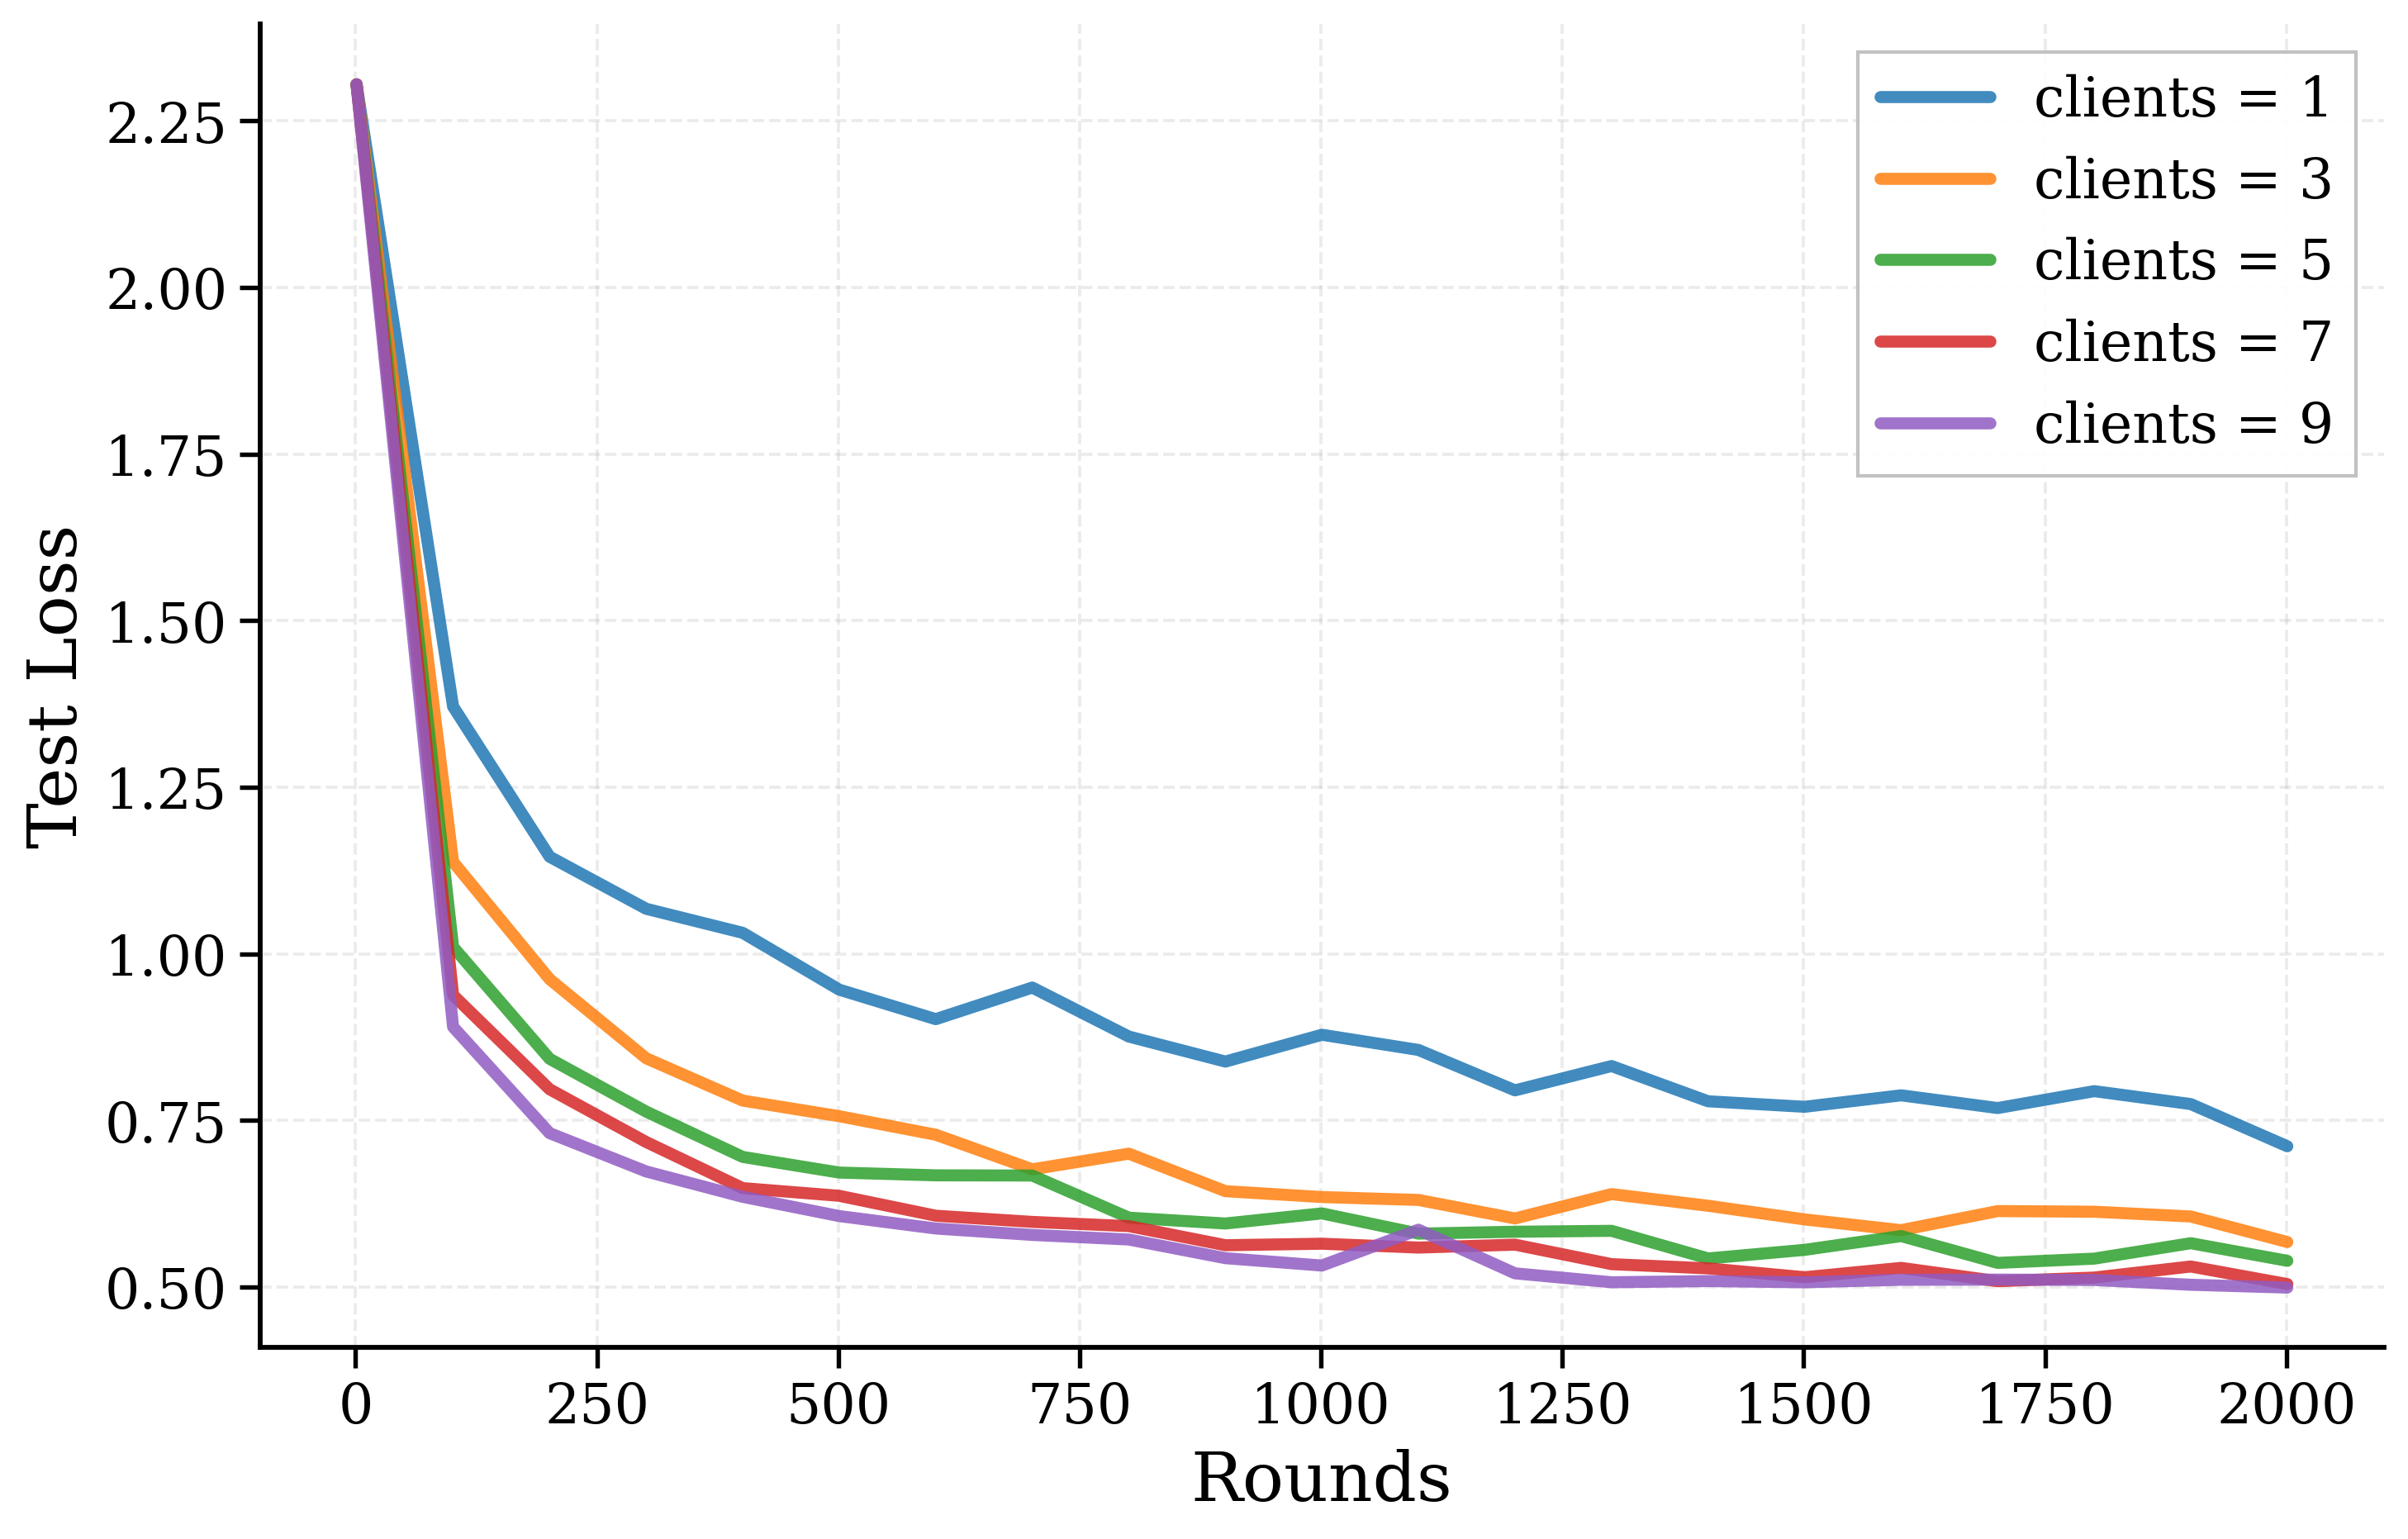
\includegraphics[width=\textwidth]{images/federated_images/signmuon_loss.png} 
        \caption{Test Loss}
    \end{subfigure}
    \hfill
    \begin{subfigure}[b]{0.48\textwidth}
        \centering
        
\includegraphics[width=\textwidth]{images/federated_images/signmuon_acc.png}
        \caption{Test Accuracy}
    \end{subfigure}
    \caption{CIFAR-10 Federated Learning. Experiment 1. Scalability of the SignMuon Algorithm.}
    \label{fig:exp_1}
\end{figure}


\subsection{Federated training results. Experiment 2}\label{app:results_fed:2}
\begin{table}[H]
\centering
\caption{CIFAR-10 Federated Learning. Experiment 2: Comparison of Optimization Algorithms with (N = 3) Clients.}
\label{tab:exp_2}
\small
\renewcommand{\arraystretch}{1.2}
\begin{tabular}{|c|c|c|c|c|c|c|c|c|}
\hline
\textbf{Dataset} & \textbf{Optimizer} & \textbf{Rounds} & \textbf{Clients} & \textbf{Steps} & \textbf{Batch} & \textbf{LR} & \textbf{Mom} & \textbf{Test Acc} \\
\hline
\multirow{6}{*}{CIFAR-10} & SignMuon & \multirow{6}{*}{2000} & \multirow{6}{*}{3} & \multirow{6}{*}{1} & \multirow{6}{*}{64} & 0.001 & \multirow{6}{*}{0.9} & 81.24\% \\
\cline{2-2} \cline{7-7} \cline{9-9}
 & Muon & & & & & 0.05 & & 81.27\% \\
\cline{2-2} \cline{7-7} \cline{9-9}
 & SignSGD & & & & & 0.001 & & 65.96\% \\
\cline{2-2} \cline{7-7} \cline{9-9}
 & SGD & & & & & 0.03 & & 76.77\% \\
\cline{2-2} \cline{7-7} \cline{9-9}
 & Adam & & & & & 0.001 & & 70.83\% \\
\cline{2-2} \cline{7-7} \cline{9-9}
 & EF-SignMuon & & & & & 0.02 & & 80.69\% \\
\hline
\end{tabular}
\end{table}

\begin{figure}[H]
    \centering
    \begin{subfigure}[b]{0.48\textwidth}
        \centering
        
\includegraphics[width=\textwidth]{images/federated_images/3_1_loss.png} 
        \caption{Test Loss}
    \end{subfigure}
    \hfill
    \begin{subfigure}[b]{0.48\textwidth}
        \centering
        
\includegraphics[width=\textwidth]{images/federated_images/3_1_acc.png}
        \caption{Test Accuracy}
    \end{subfigure}
    \caption{CIFAR-10 Federated Learning. Experiment 2: Comparison of Optimization Algorithms with (N = 3) Clients.}
    \label{fig:exp_2}
\end{figure}

\subsection{Federated training results. Experiment 3}\label{app:results_fed:3}
\begin{figure}[H]
    \centering
    \begin{subfigure}[b]{0.48\textwidth}
        \centering
        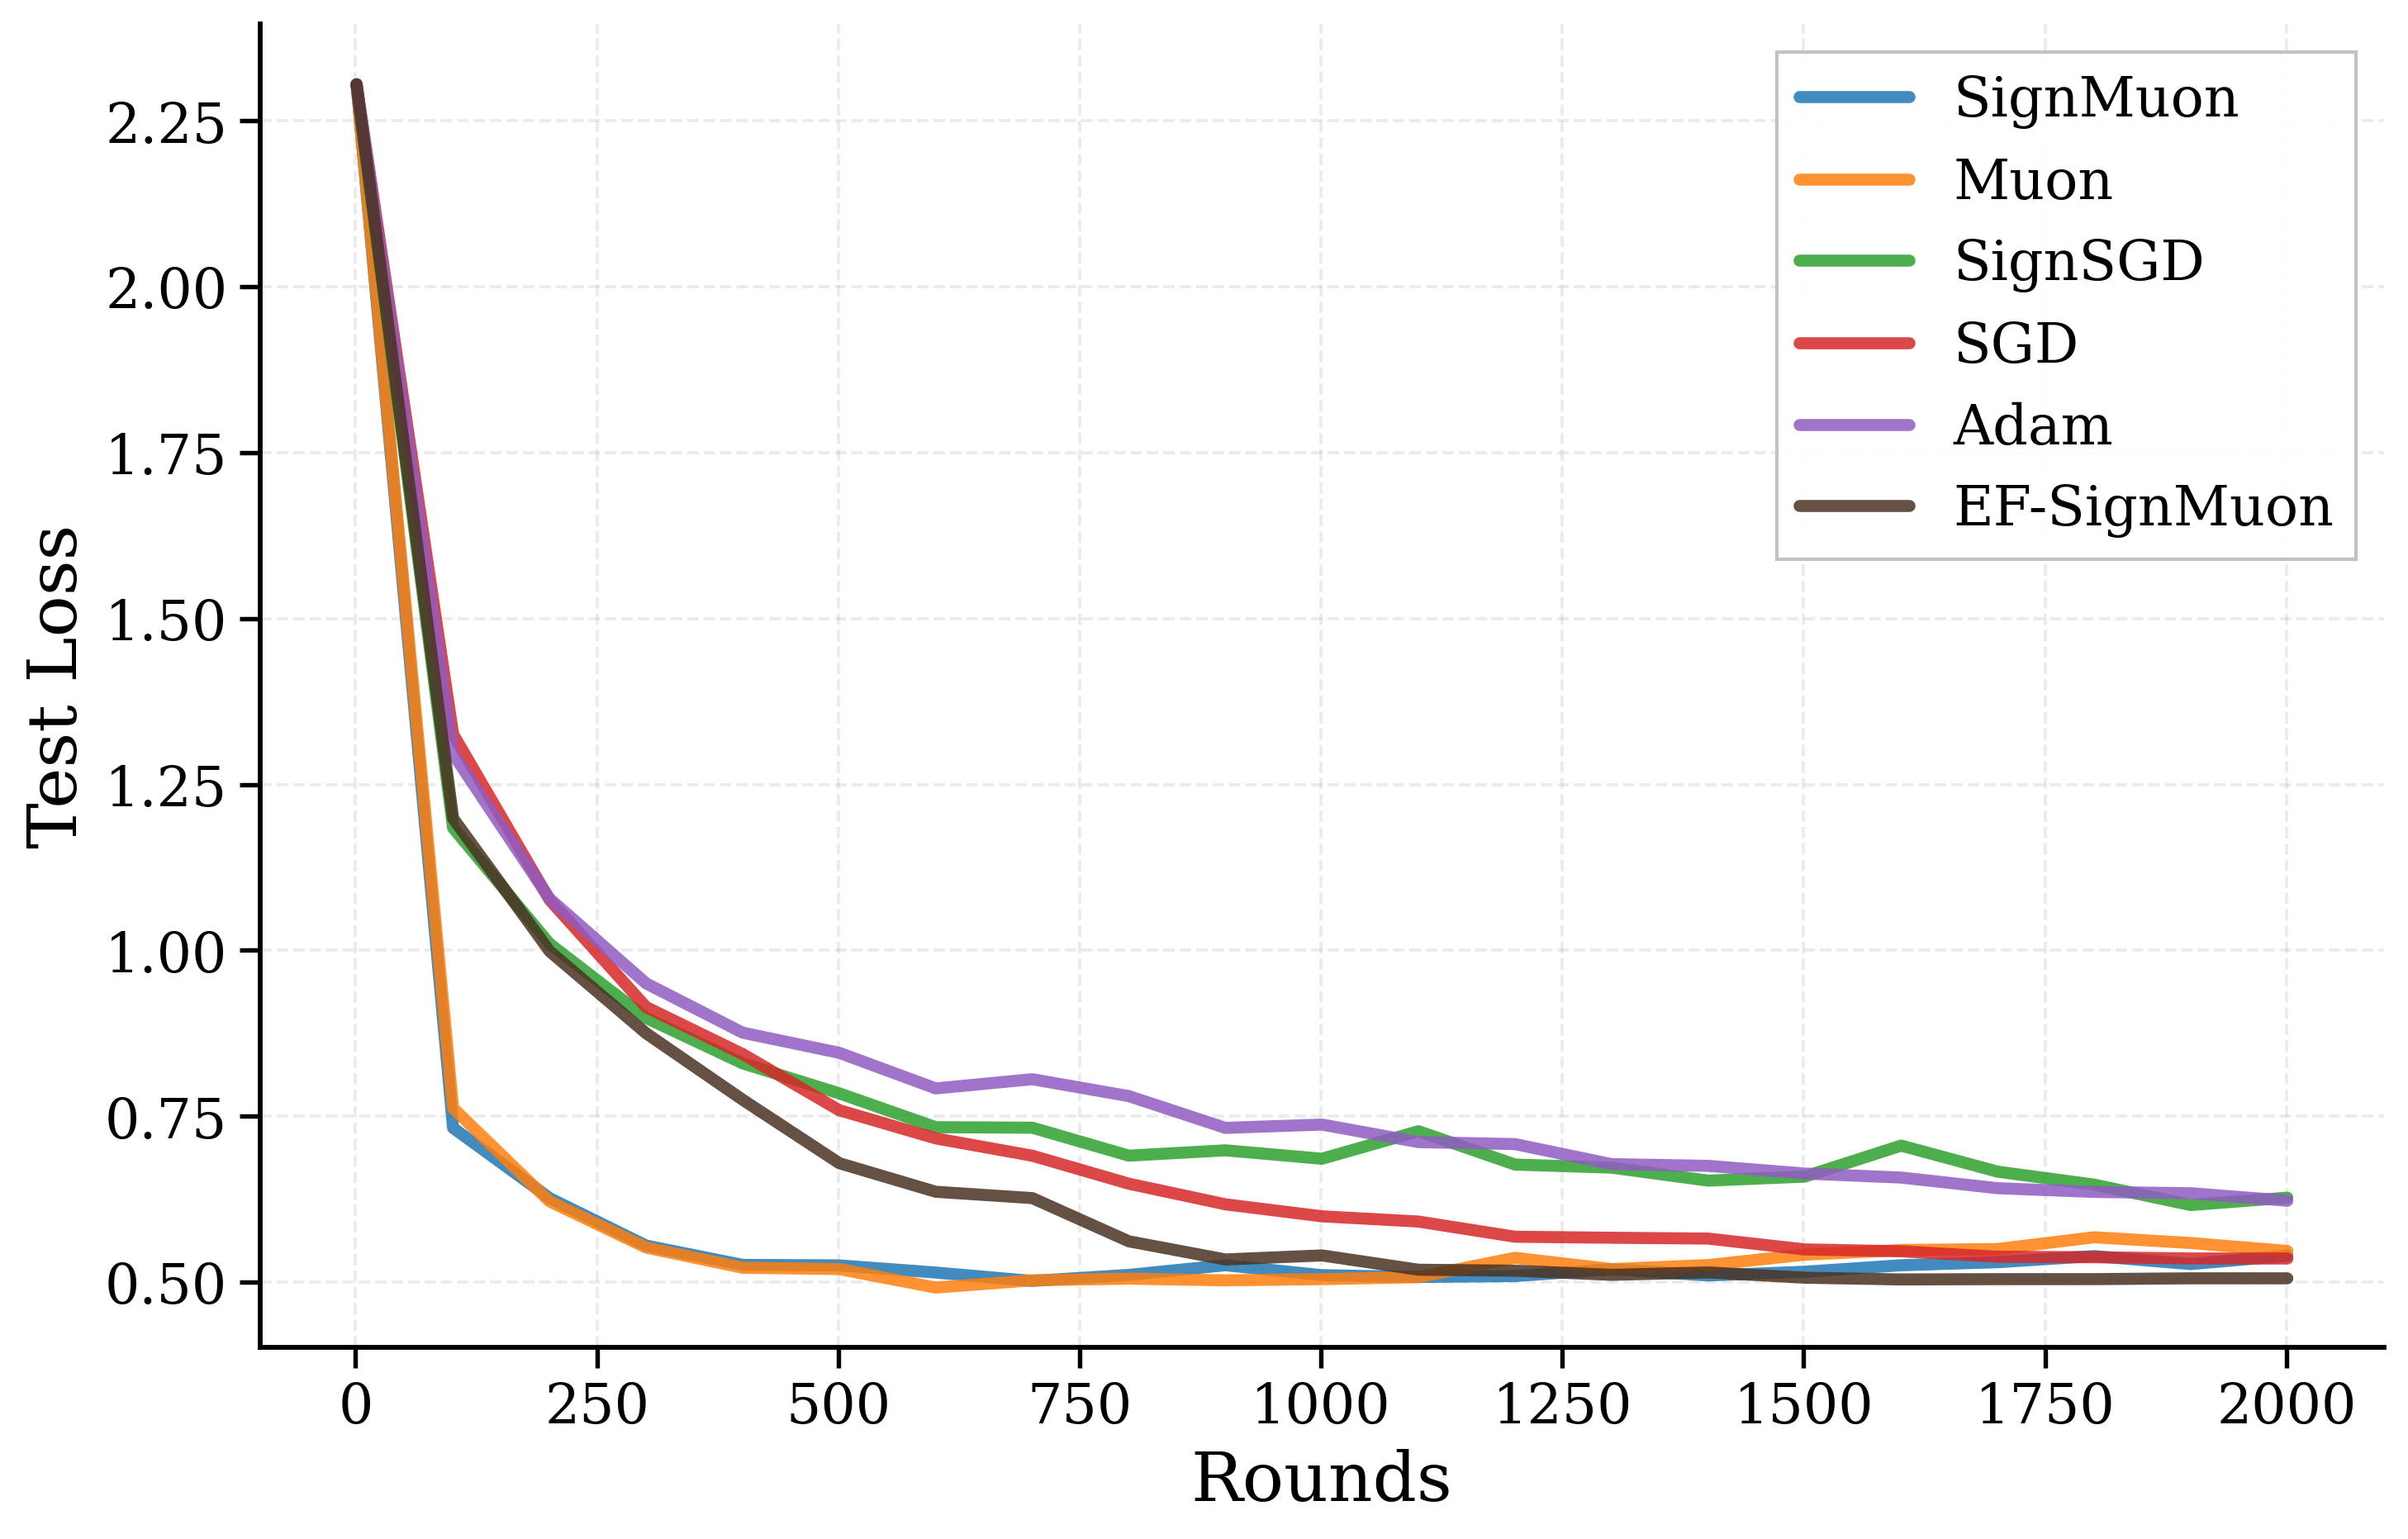
\includegraphics[width=\textwidth]{images/federated_images/10_3_loss.png} 
        \caption{Test Loss}
    \end{subfigure}
    \hfill
    \begin{subfigure}[b]{0.48\textwidth}
        \centering
        
\includegraphics[width=\textwidth]{images/federated_images/10_3_acc.png}
        \caption{Test Accuracy}
    \end{subfigure}
    \caption{CIFAR-10 Federated Learning. Experiment 3: Comparison of Optimization Algorithms with (N = 10) Clients.}
    \label{fig:exp_3}
\end{figure}


\end{document}